\section{Resultados}

\begin{frame}{Resultados}
    \begin{itemize}
        \item Front-end: Protótipos
    \end{itemize}
    \begin{minipage}{0.48\textwidth}
        \centering
        \captionof{figure}{Protótipo da tela inicial}
        
\includegraphics[width=1\textwidth]{figuras/proto-1.png}
        \footnotesize Fonte: Elaborado pelo autor (2024)
    \end{minipage}
    \hfill
    \begin{minipage}{0.48\textwidth}
        \centering
        \captionof{figure}{Protótipo da tela dos cursos}
        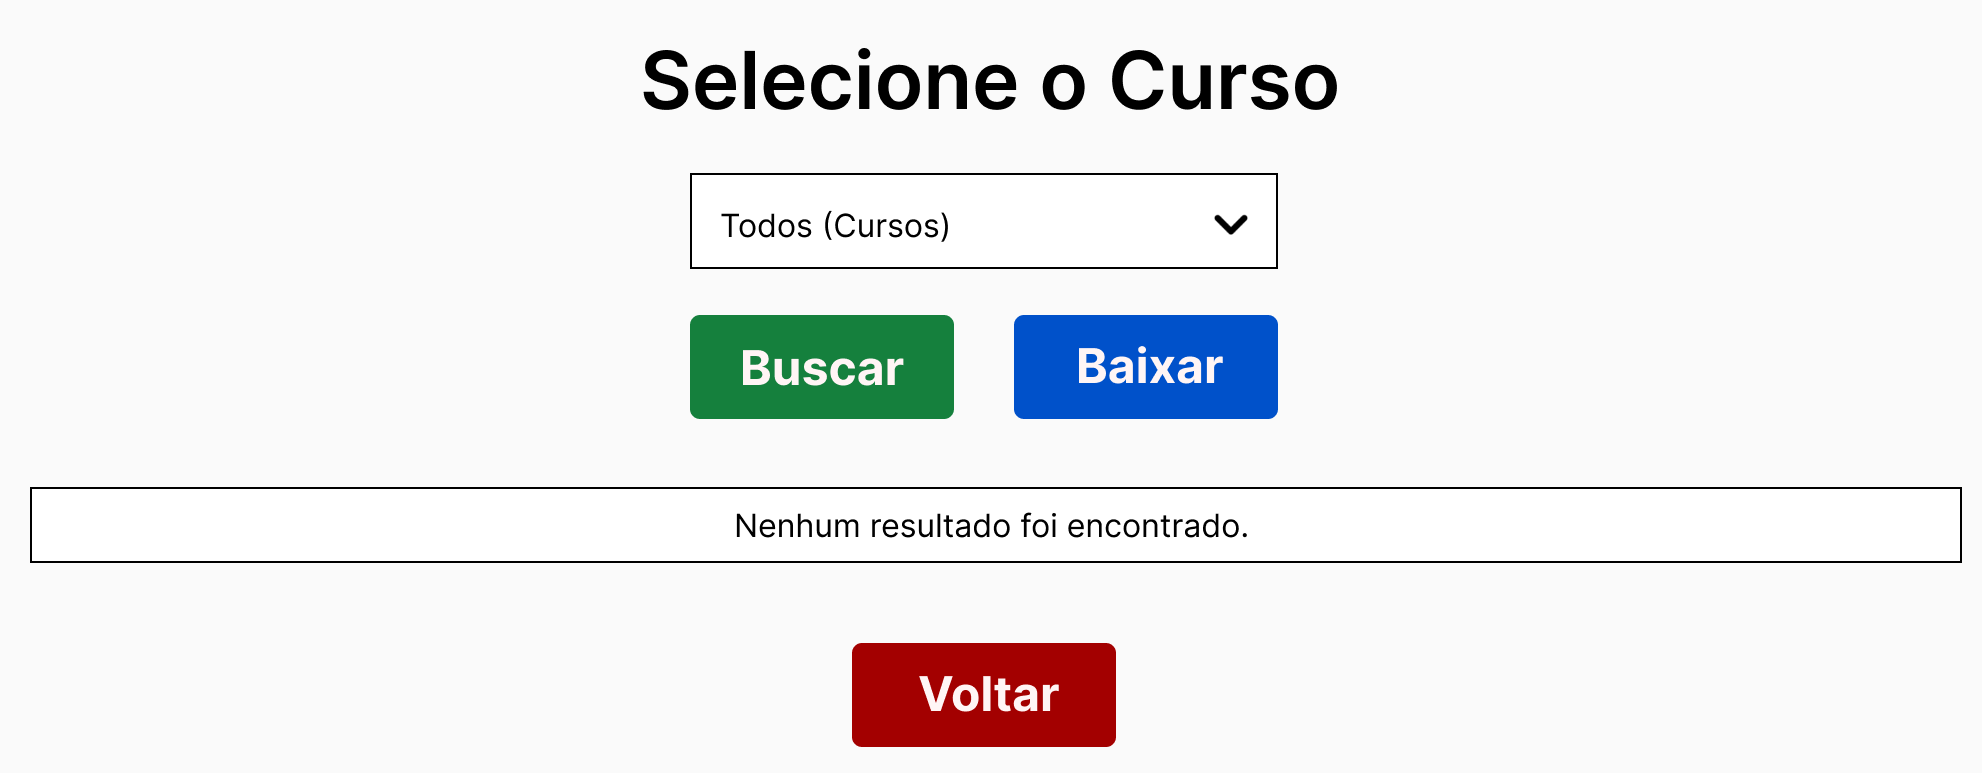
\includegraphics[width=1\textwidth]{figuras/proto-2.png}
        \footnotesize Fonte: Elaborado pelo autor (2024)
    \end{minipage}
\end{frame}

\begin{frame}{Protótipos}
    \begin{minipage}{0.48\textwidth}
        \centering
        \captionof{figure}{Protótipo da tela dos cursos preenchida}
        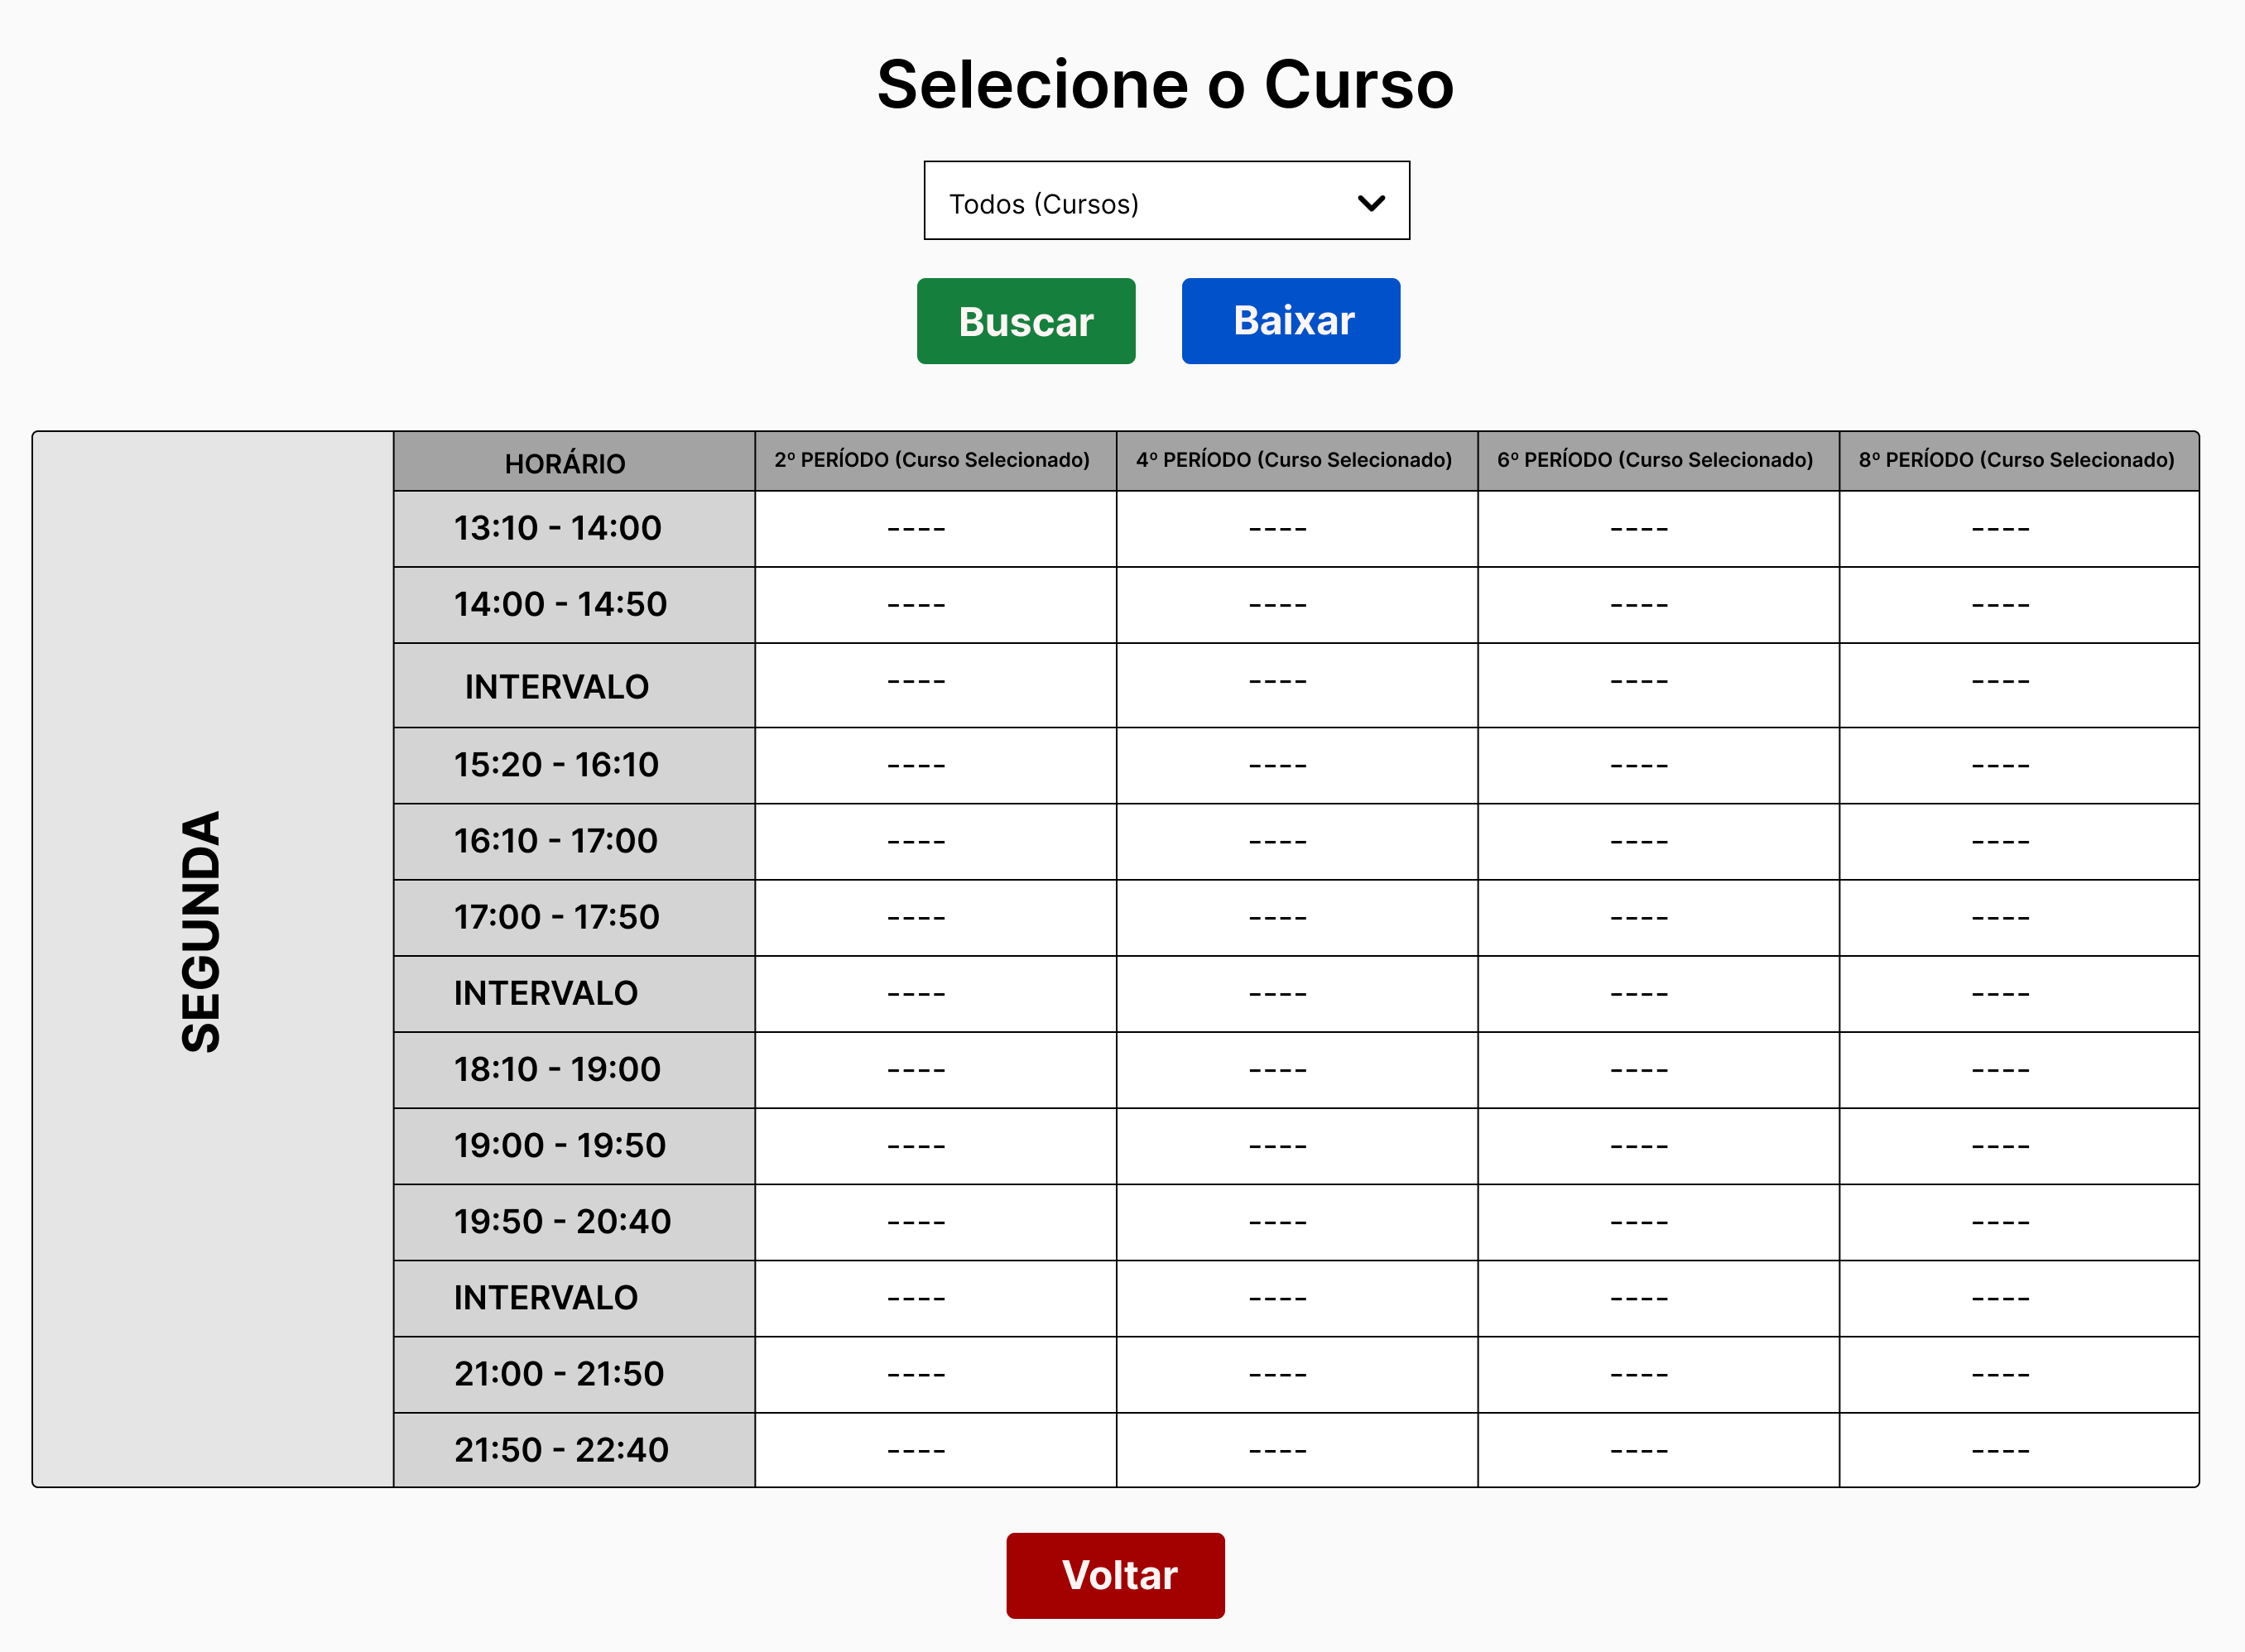
\includegraphics[width=1\textwidth]{figuras/proto-3.png}
        \footnotesize Fonte: Elaborado pelo autor (2024)
    \end{minipage}
    \hfill
    \begin{minipage}{0.48\textwidth}
        \centering
        \captionof{figure}{Protótipo da tela dos professores}
        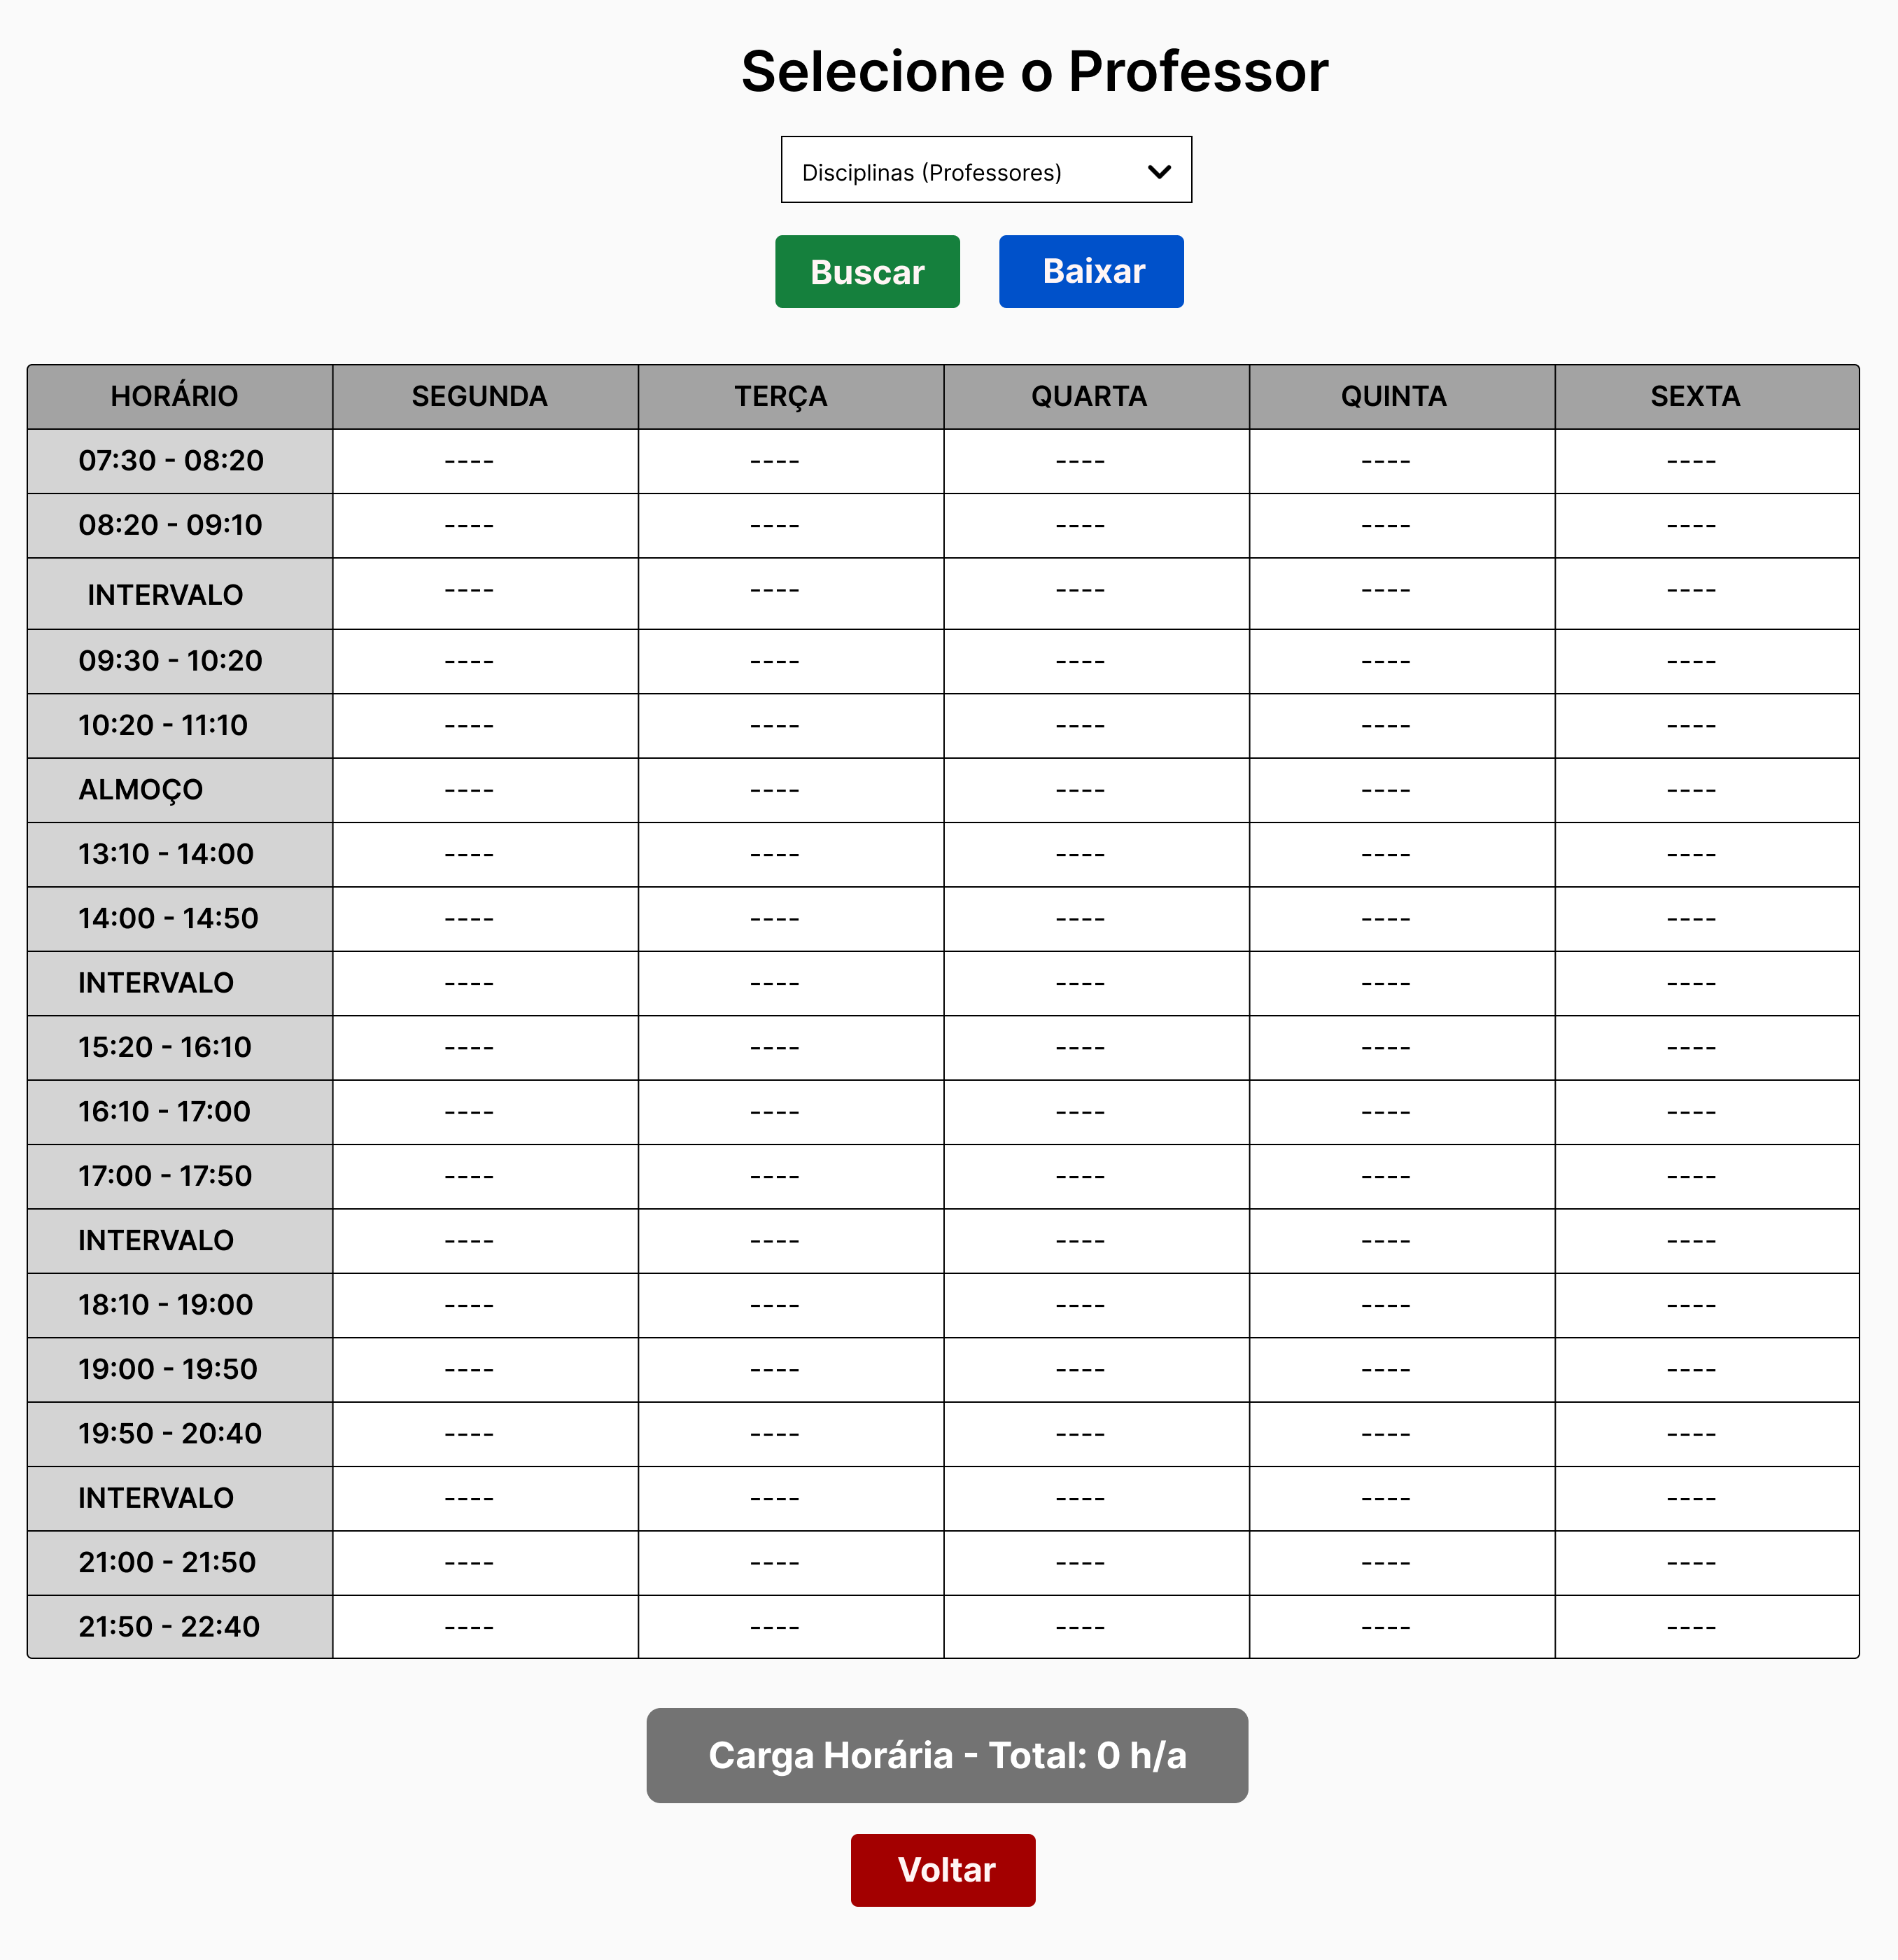
\includegraphics[width=0.9\textwidth]{figuras/proto-4.png}
        \footnotesize Fonte: Elaborado pelo autor (2024)
    \end{minipage}
\end{frame}

\begin{frame}{Protótipos}
    \begin{figure}
        \centering
        \vspace{-0.5cm}
        \caption{Protótipo da tela das salas}
        \vspace{-0.2cm}
        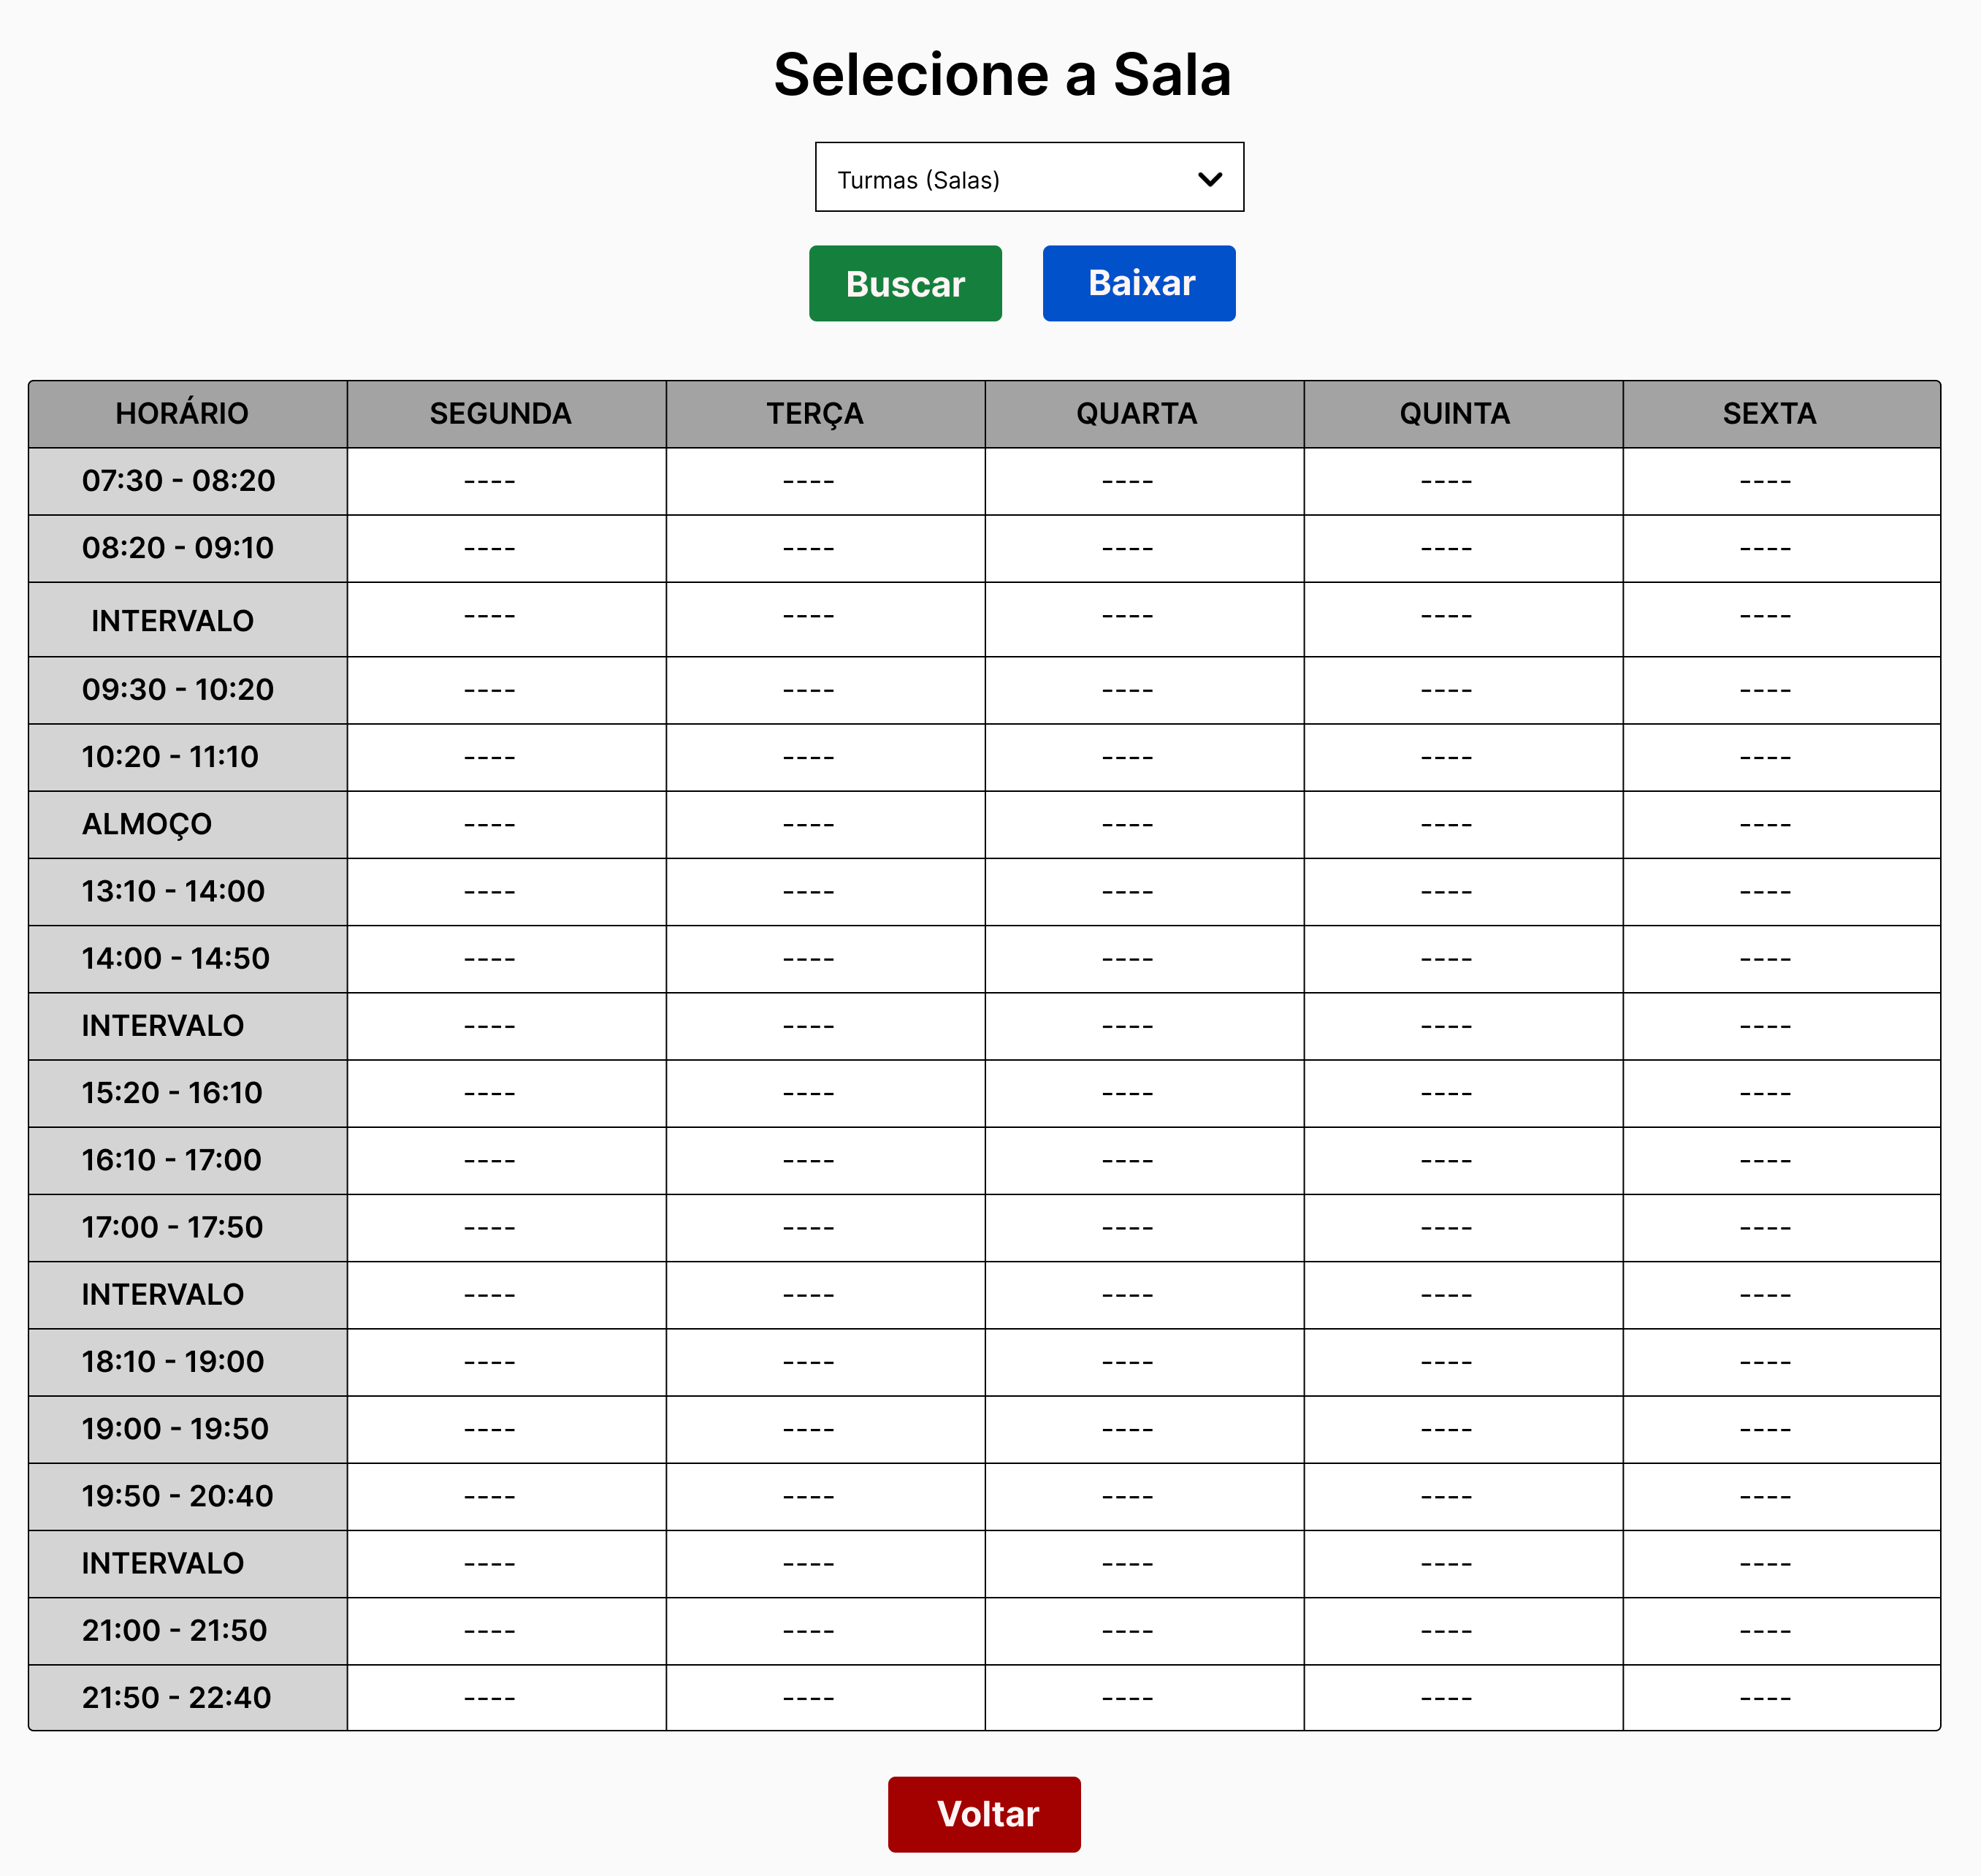
\includegraphics[width=0.75\textwidth]{figuras/proto-5.png}
        \\ % Quebra de linha para separar a imagem da fonte
        \footnotesize Fonte: Elaborado pelo autor (2024)
    \end{figure}
\end{frame}

\begin{frame}{Desenvolvimento do Front-end}
    \begin{minipage}{0.48\textwidth}
        \centering
        \captionof{figure}{Menu principal com opções de botões de horários e outros serviços}
        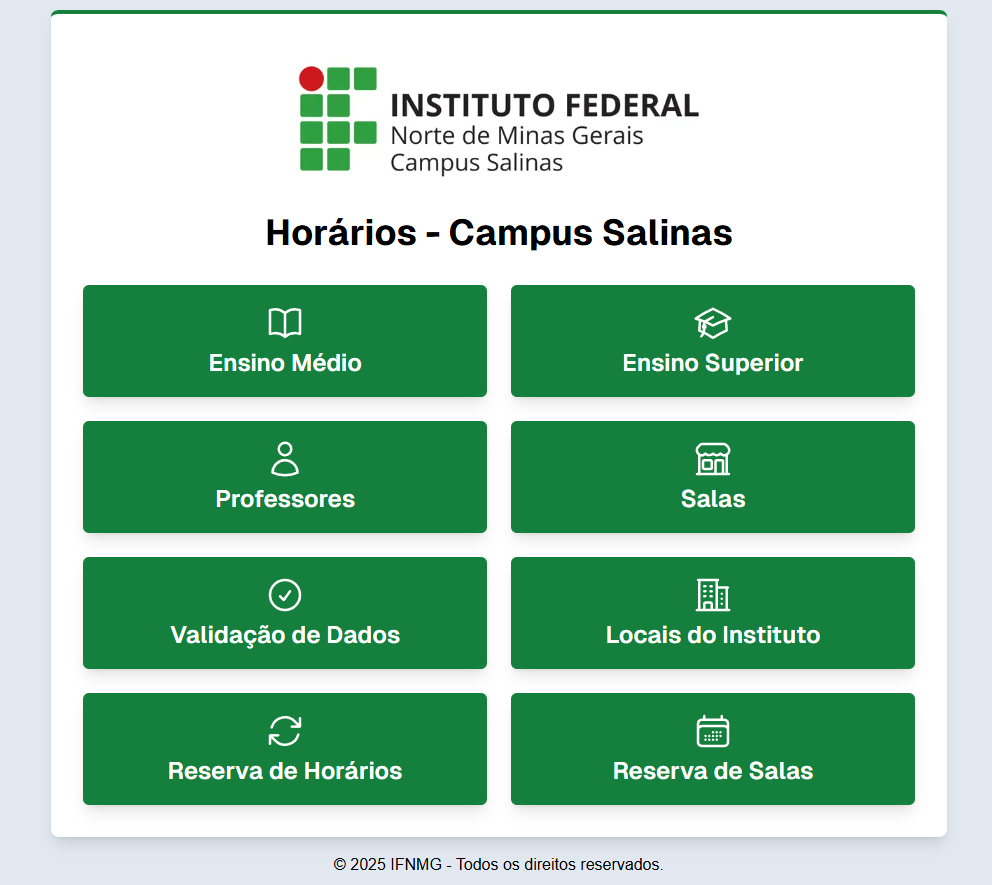
\includegraphics[width=0.9\textwidth]{figuras/front-1.png}
        \footnotesize Fonte: Elaborado pelo autor (2025)
    \end{minipage}
    \hfill
    \begin{minipage}{0.48\textwidth}
        \centering
        \captionof{figure}{Tela dos cursos}
        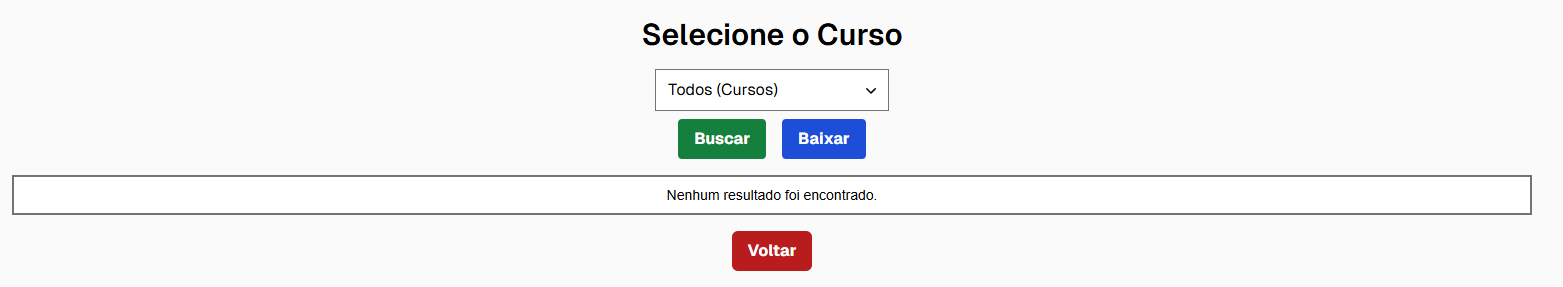
\includegraphics[width=1\textwidth]{figuras/front-2.png}
        \footnotesize Fonte: Elaborado pelo autor (2025)
    \end{minipage}
\end{frame}

\begin{frame}{Desenvolvimento do Front-end}
    \begin{minipage}{0.48\textwidth}
        \centering
        \captionof{figure}{Tela dos cursos com cursos técnicos}
        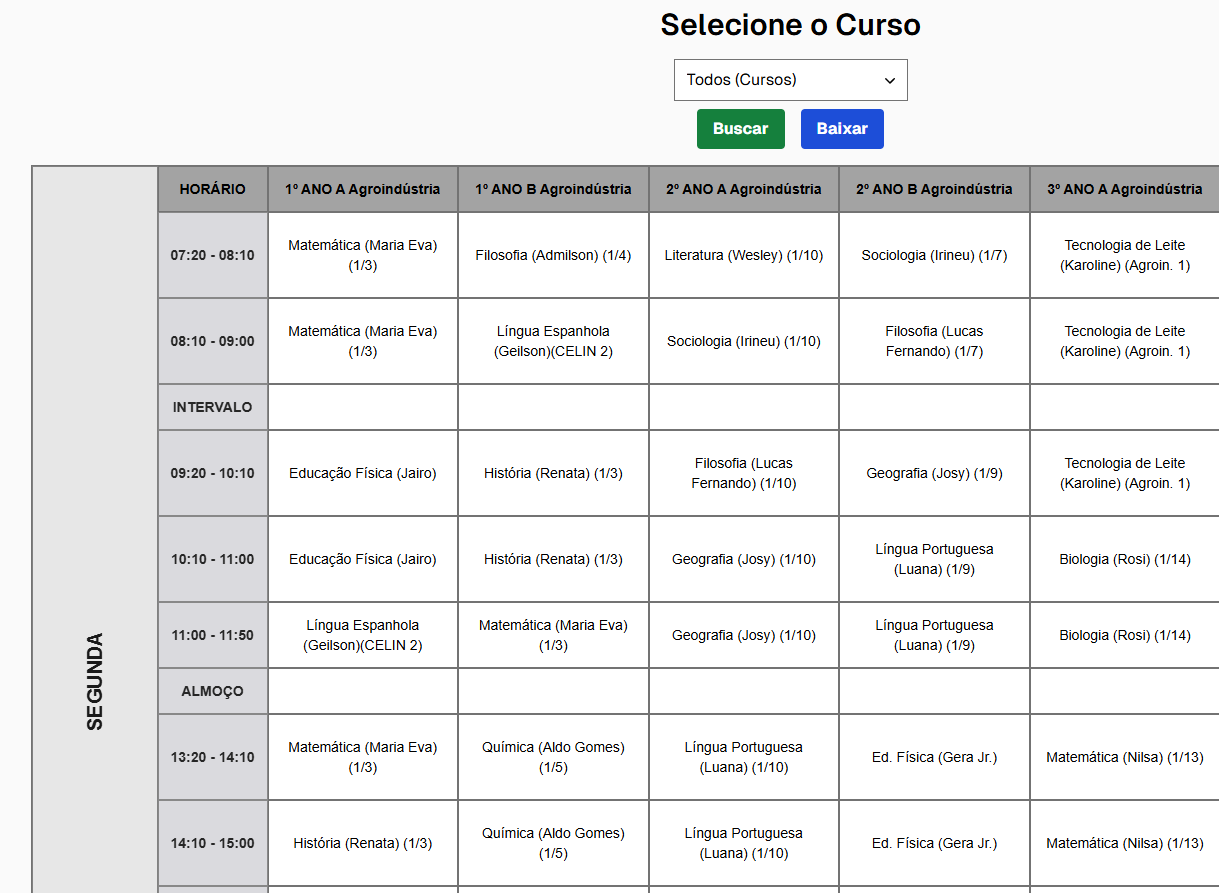
\includegraphics[width=1\textwidth]{figuras/front-3.png}
        \footnotesize Fonte: Elaborado pelo autor (2025)
    \end{minipage}
    \hfill
    \begin{minipage}{0.48\textwidth}
        \centering
        \captionof{figure}{Tela dos cursos com cursos superiores}
        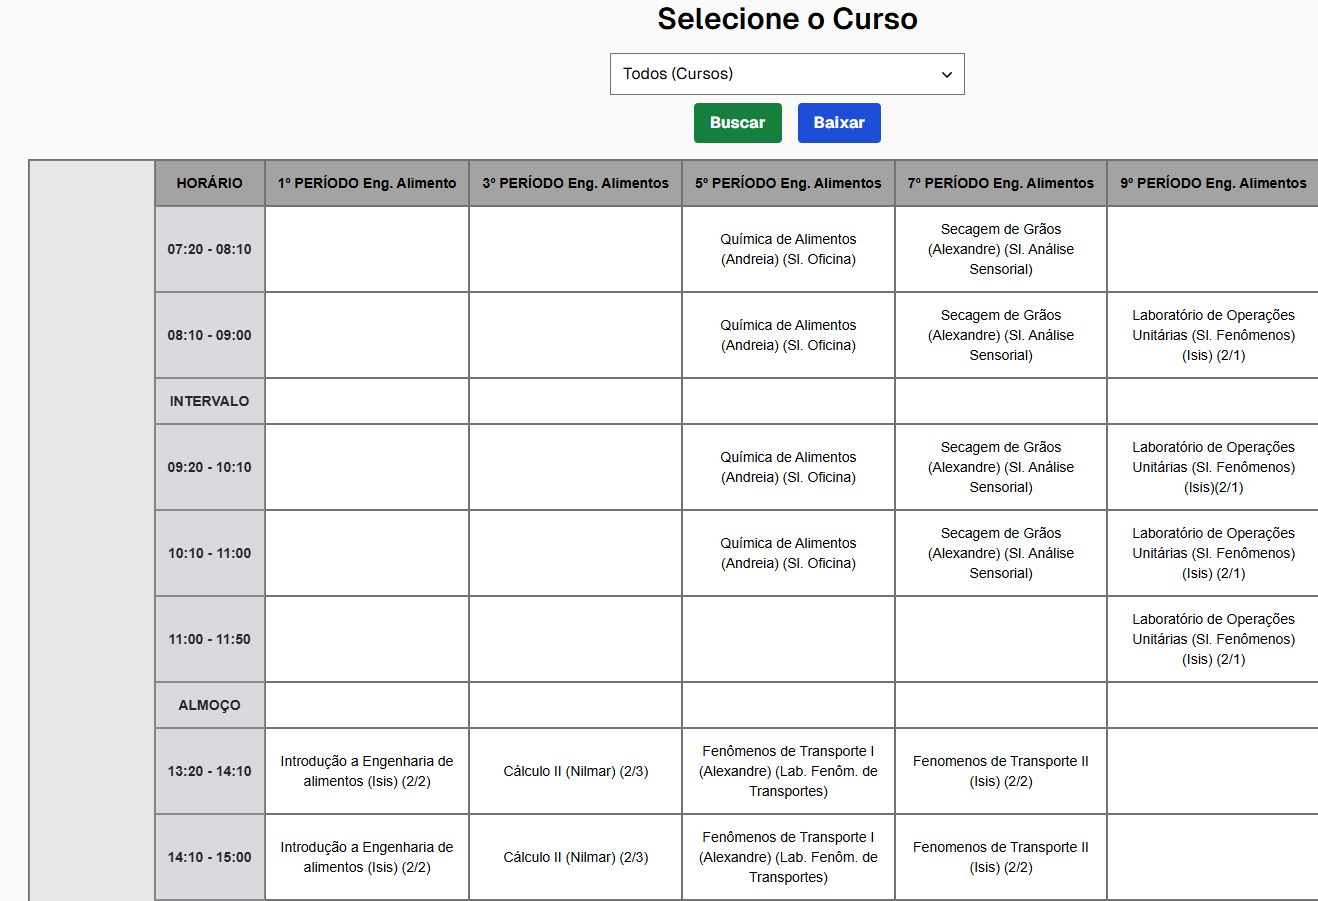
\includegraphics[width=1\textwidth]{figuras/front-4.png}
        \footnotesize Fonte: Elaborado pelo autor (2025)
    \end{minipage}
\end{frame}

\begin{frame}{Desenvolvimento do Front-end}
    \begin{minipage}{0.48\textwidth}
        \centering
        \captionof{figure}{Tela dos professores}
        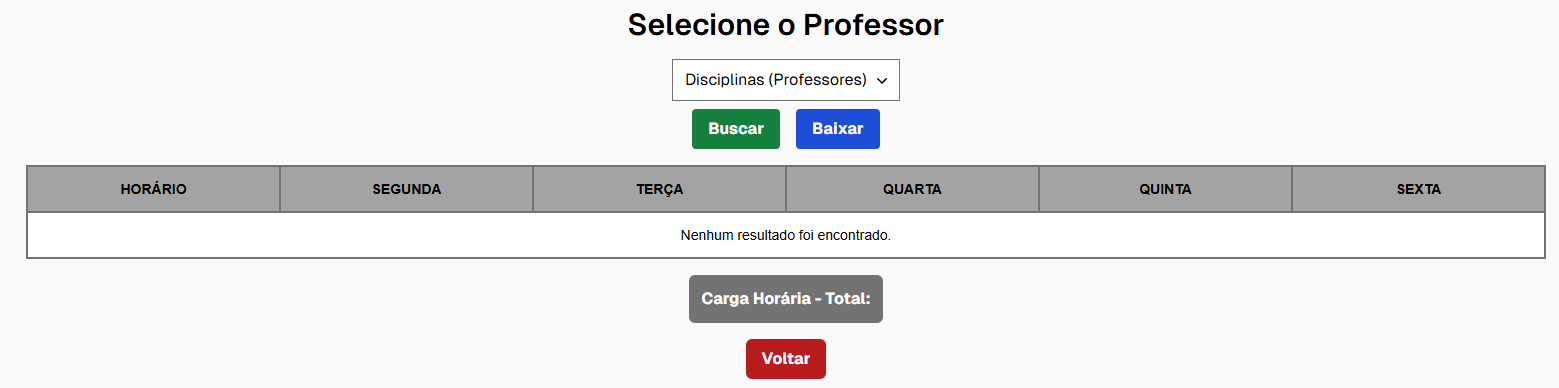
\includegraphics[width=1\textwidth]{figuras/front-5.png}
        \footnotesize Fonte: Elaborado pelo autor (2025)
    \end{minipage}
    \hfill
    \begin{minipage}{0.48\textwidth}
        \centering
        \captionof{figure}{Tela dos professores com um professor selecionado}
        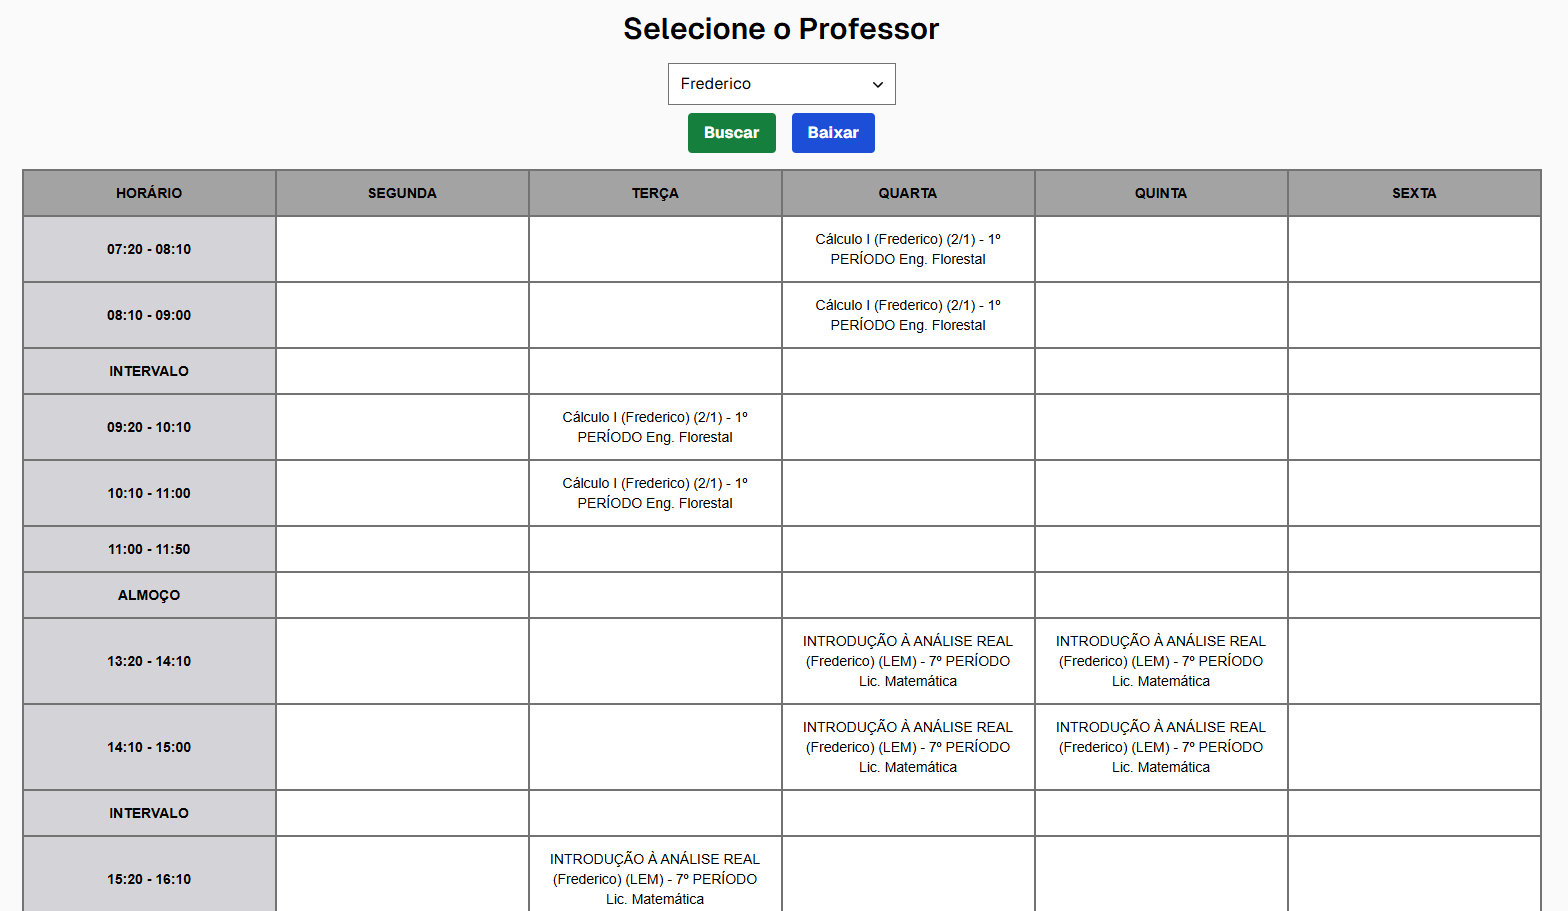
\includegraphics[width=1\textwidth]{figuras/front-6.png}
        \footnotesize Fonte: Elaborado pelo autor (2025)
    \end{minipage}
\end{frame}

\begin{frame}{Desenvolvimento do Front-end}
    \begin{minipage}{0.48\textwidth}
        \centering
        \captionof{figure}{Tela das salas}
        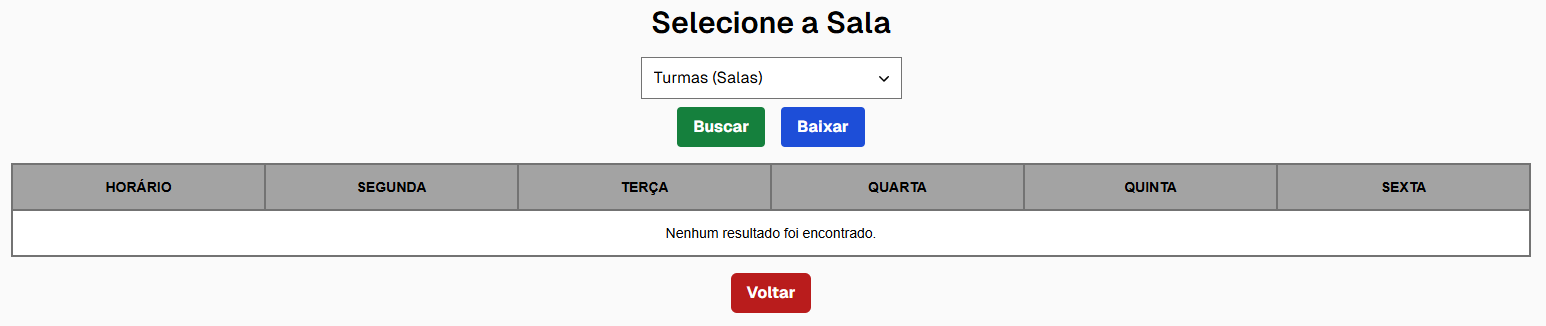
\includegraphics[width=1\textwidth]{figuras/front-7.png}
        \footnotesize Fonte: Elaborado pelo autor (2025)
    \end{minipage}
    \hfill
    \begin{minipage}{0.48\textwidth}
        \centering
        \captionof{figure}{Tela das salas com uma sala selecionada}
        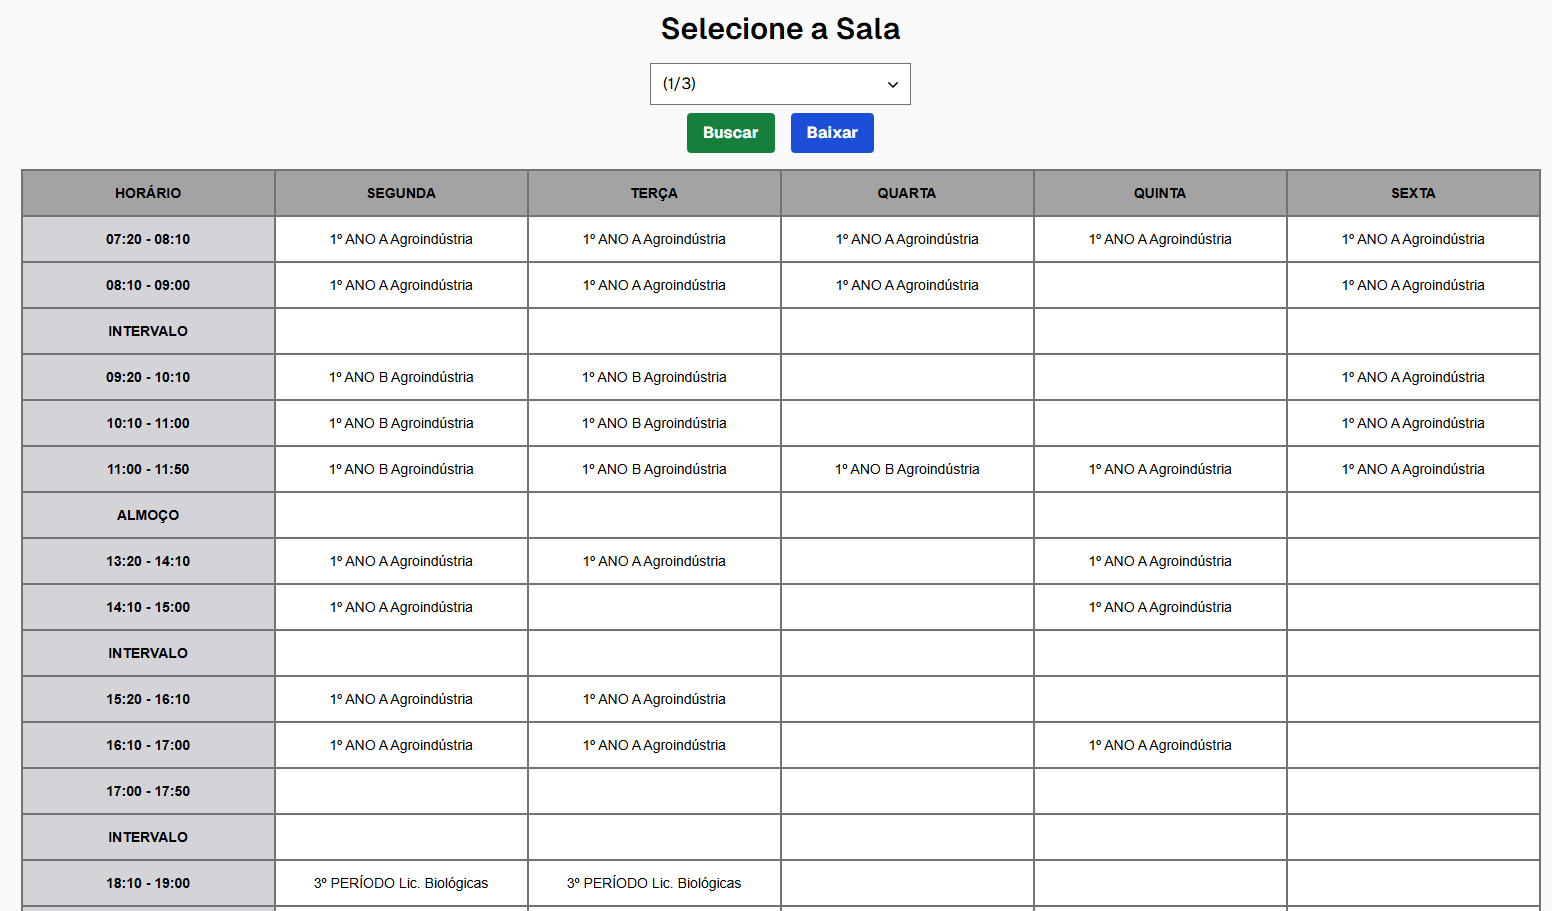
\includegraphics[width=1\textwidth]{figuras/front-8.png}
        \footnotesize Fonte: Elaborado pelo autor (2025)
    \end{minipage}
\end{frame}

\begin{frame}{Desenvolvimento do Front-end}
    \begin{figure}
        \centering
        \vspace{-0.5cm}
        \caption{Tela de login}
        \vspace{-0.2cm}
        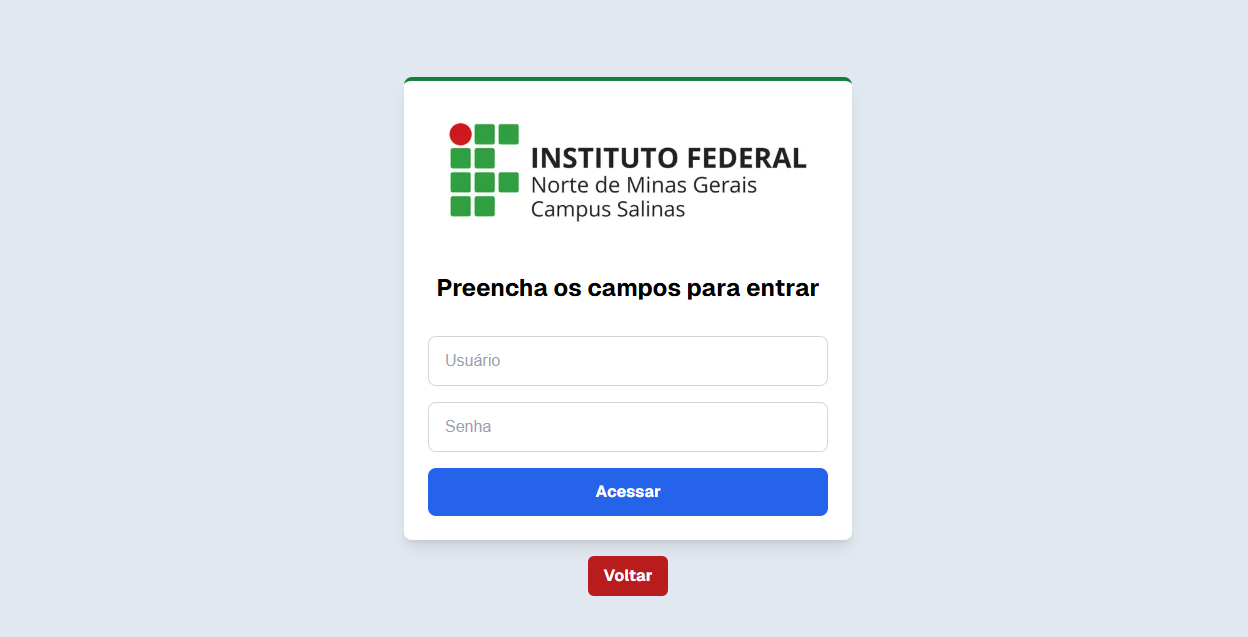
\includegraphics[width=1\textwidth]{figuras/front-9.png}
        \\ % Quebra de linha para separar a imagem da fonte
        \footnotesize Fonte: Elaborado pelo autor (2025)
    \end{figure}
\end{frame}

\begin{frame}{Desenvolvimento do Front-end}
    \begin{figure}
        \centering
        \vspace{-0.5cm}
        \caption{Tela de validação de dados}
        \vspace{-0.2cm}
        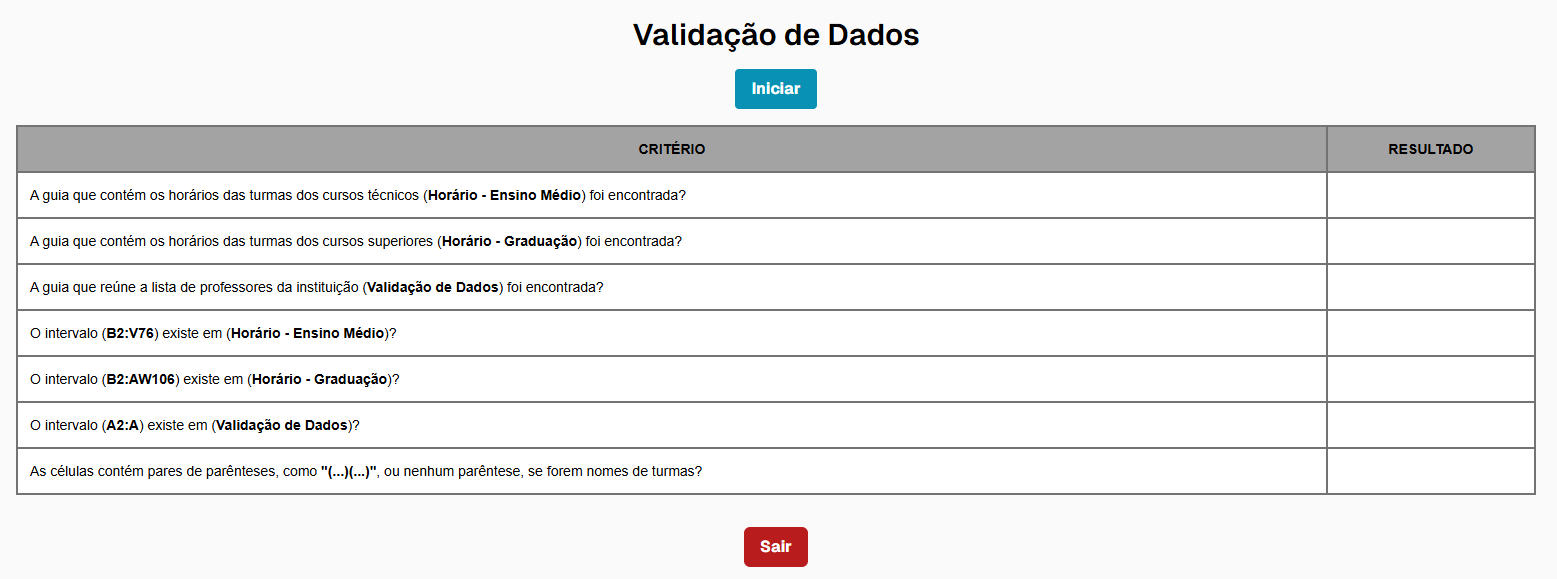
\includegraphics[width=1\textwidth]{figuras/front-10.png}
        \\ % Quebra de linha para separar a imagem da fonte
        \footnotesize Fonte: Elaborado pelo autor (2025)
    \end{figure}
\end{frame}

\begin{frame}{Desenvolvimento do Front-end}
    \begin{minipage}{0.48\textwidth}
        \centering
        \captionof{figure}{Sistema que exibe os locais do instituto}
        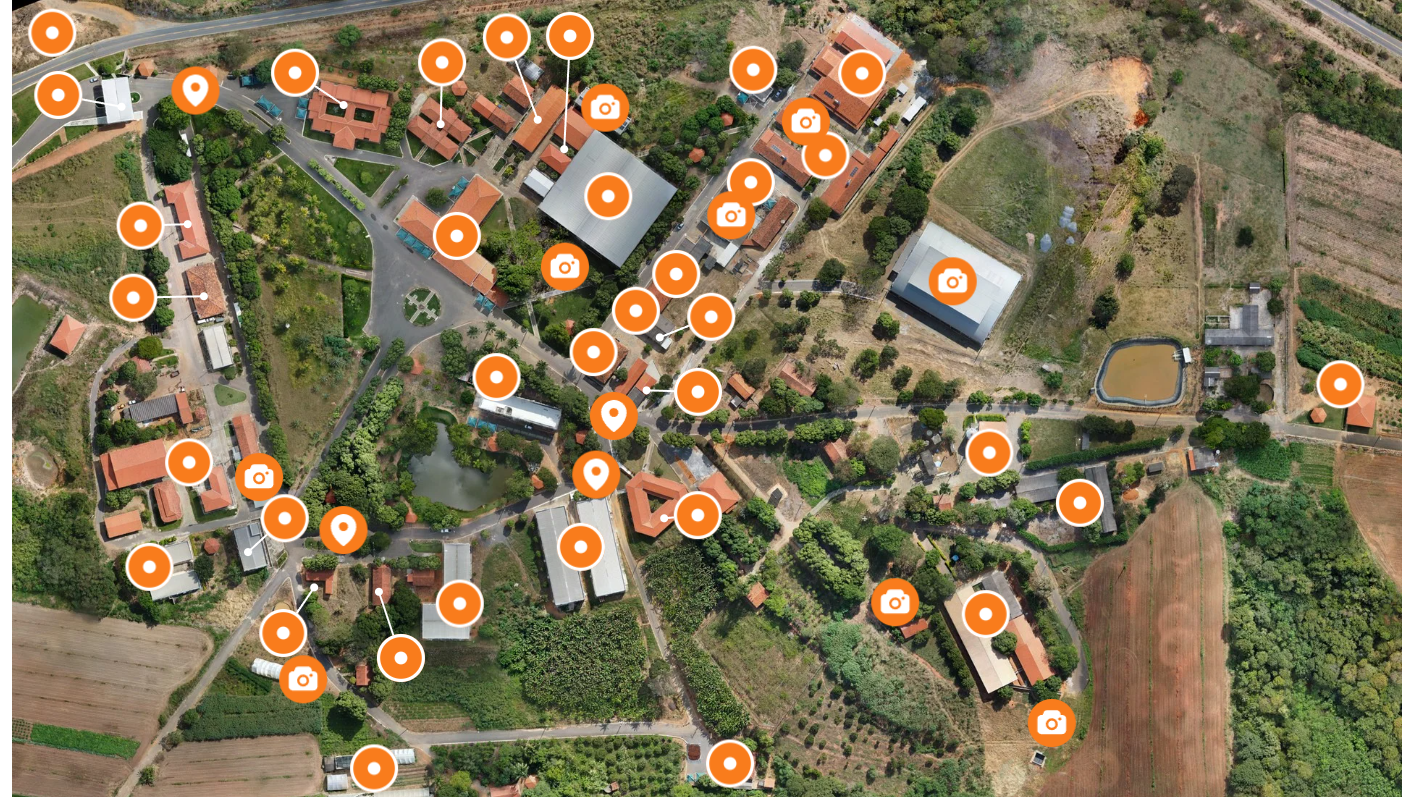
\includegraphics[width=1\textwidth]{figuras/front-11.png}
        \footnotesize Fonte: Elaborado pelo autor (2025)
    \end{minipage}
    \hfill
    \begin{minipage}{0.48\textwidth}
        \centering
        \captionof{figure}{Sistema de reserva de horários}
        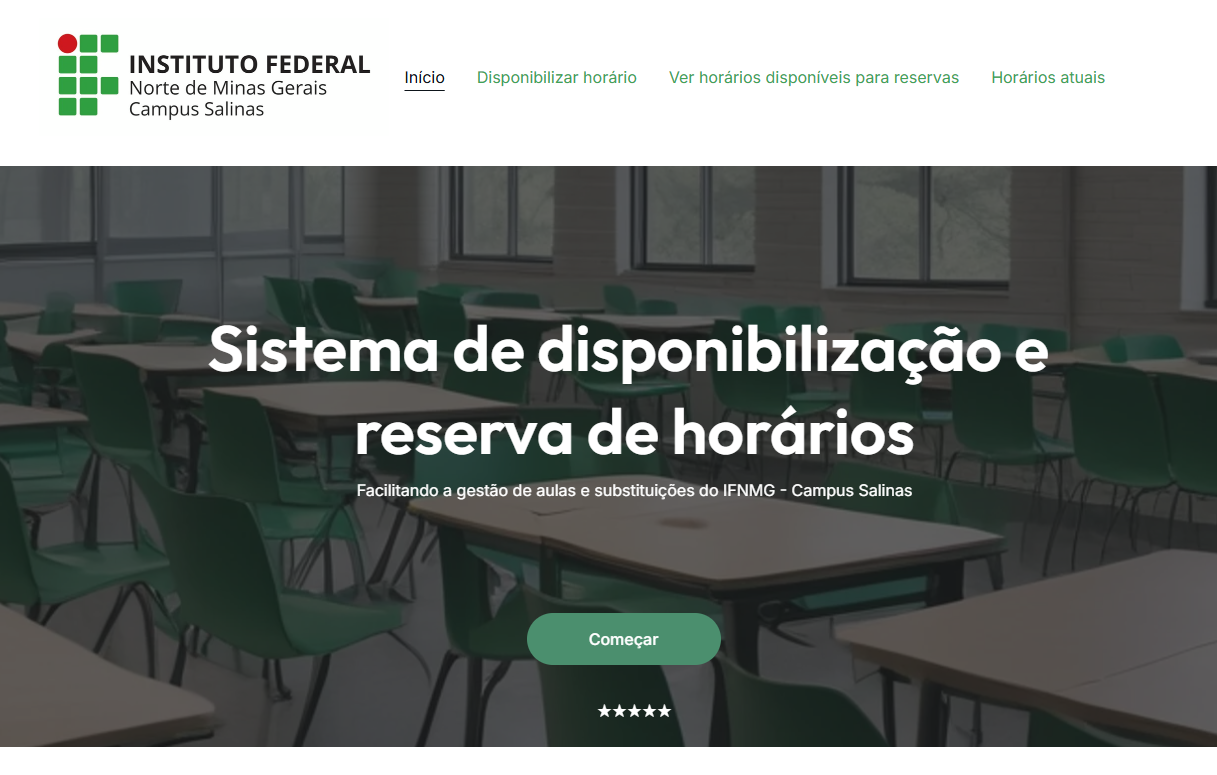
\includegraphics[width=1\textwidth]{figuras/front-12.png}
        \footnotesize Fonte: Elaborado pelo autor (2025)
    \end{minipage}
\end{frame}

\begin{frame}{Desenvolvimento do Front-end}
    \begin{figure}
        \centering
        \vspace{-0.5cm}
        \caption{Sistema de gerenciamento de reserva de salas}
        \vspace{-0.2cm}
        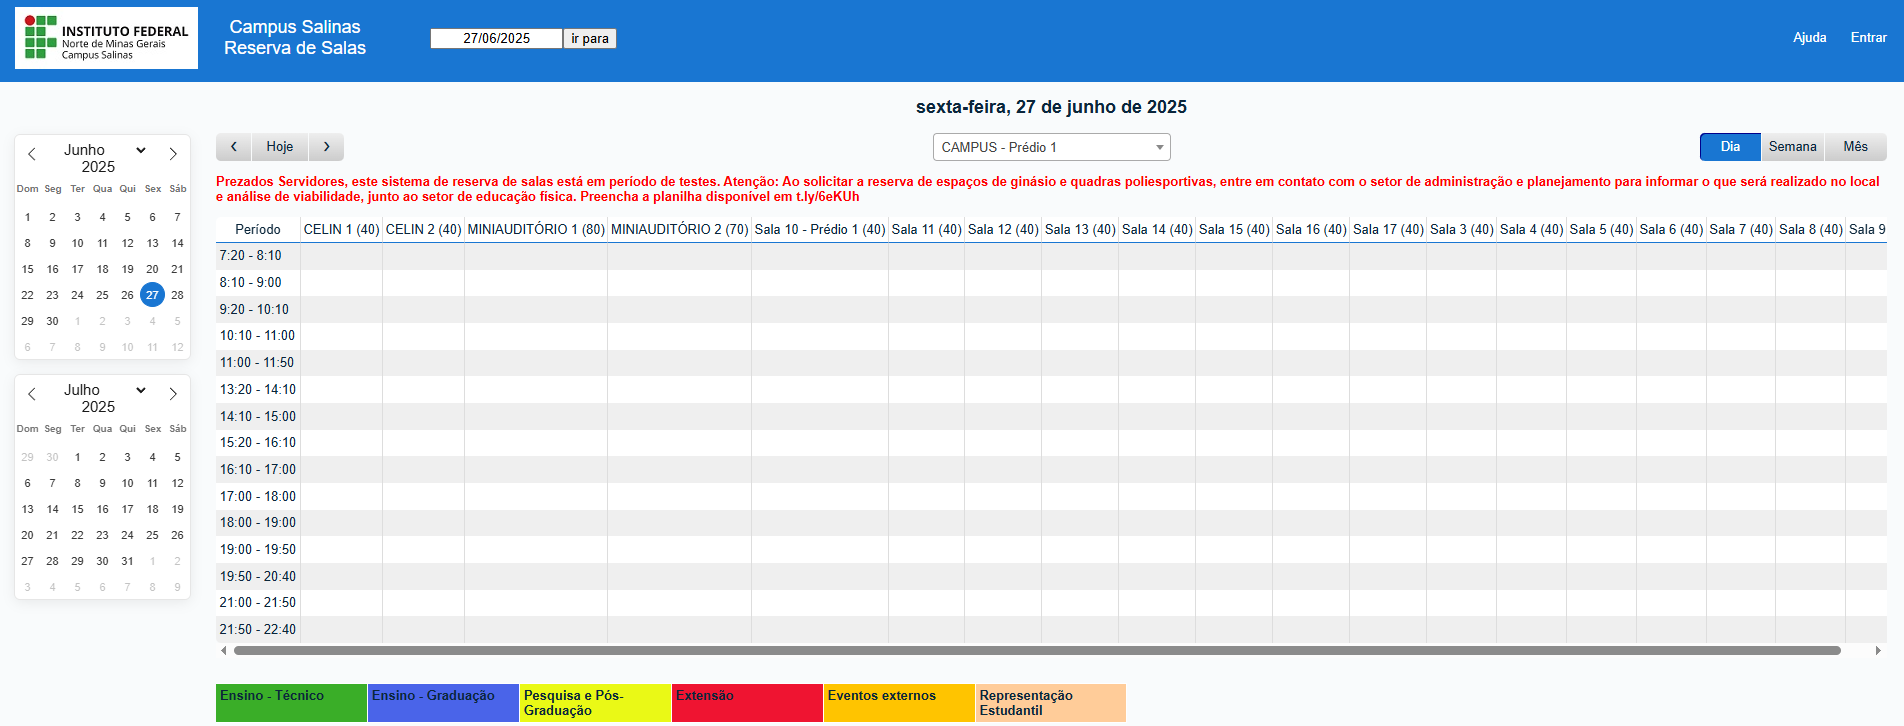
\includegraphics[width=1\textwidth]{figuras/front-13.png}
        \\ % Quebra de linha para separar a imagem da fonte
        \footnotesize Fonte: Elaborado pelo autor (2025)
    \end{figure}
\end{frame}

\begin{frame}{Estrutura do Front-end}
    \begin{figure}
        \centering
        \vspace{-0.5cm}
        \caption{Estrutura do front-end}
        \vspace{-0.2cm}
        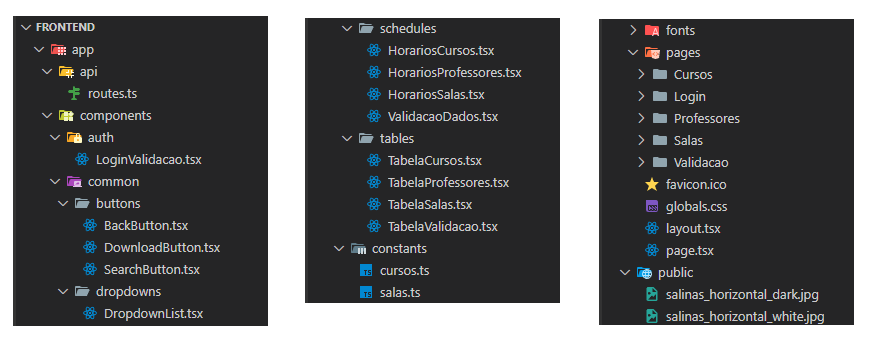
\includegraphics[width=1\textwidth]{figuras/front-14.png}
        \\ % Quebra de linha para separar a imagem da fonte
        \footnotesize Fonte: Elaborado pelo autor (2025)
    \end{figure}
\end{frame}

\begin{frame}{Funcionalidades do Front-end}
    \begin{minipage}{0.48\textwidth}
        \centering
        \captionof{figure}{Modo escuro}
        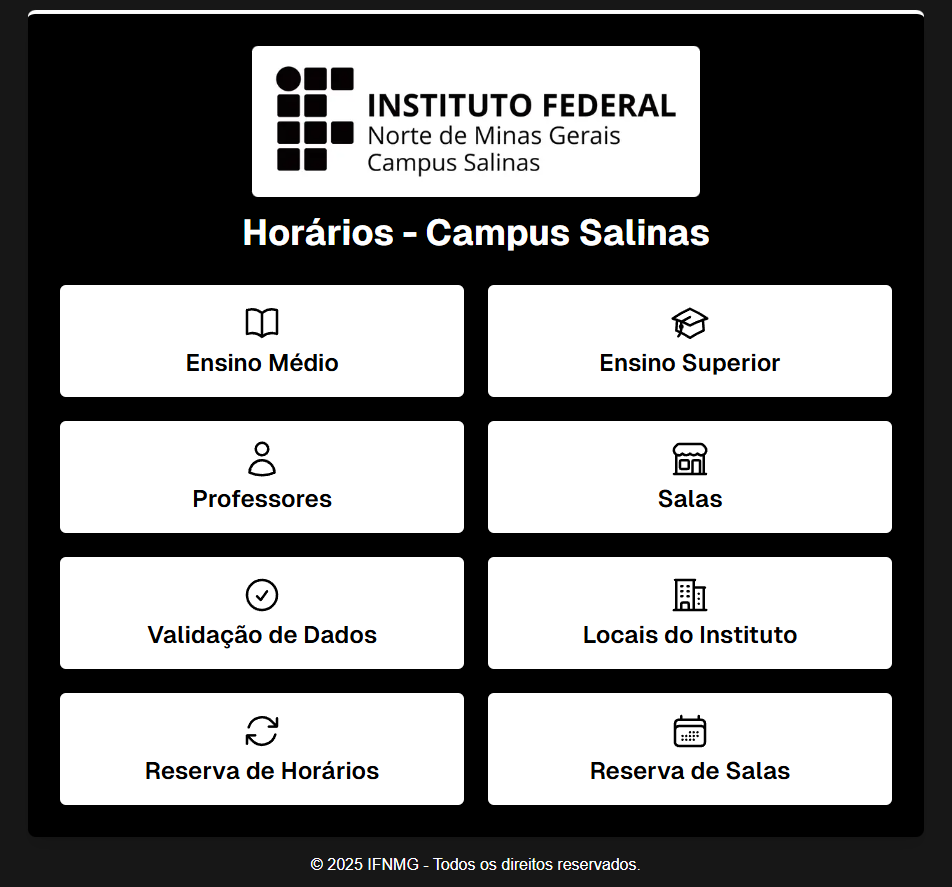
\includegraphics[width=1\textwidth]{figuras/front-15.png}
        \footnotesize Fonte: Elaborado pelo autor (2025)
    \end{minipage}
    \hfill
    \begin{minipage}{0.48\textwidth}
        \centering
        \captionof{figure}{Responsividade}
        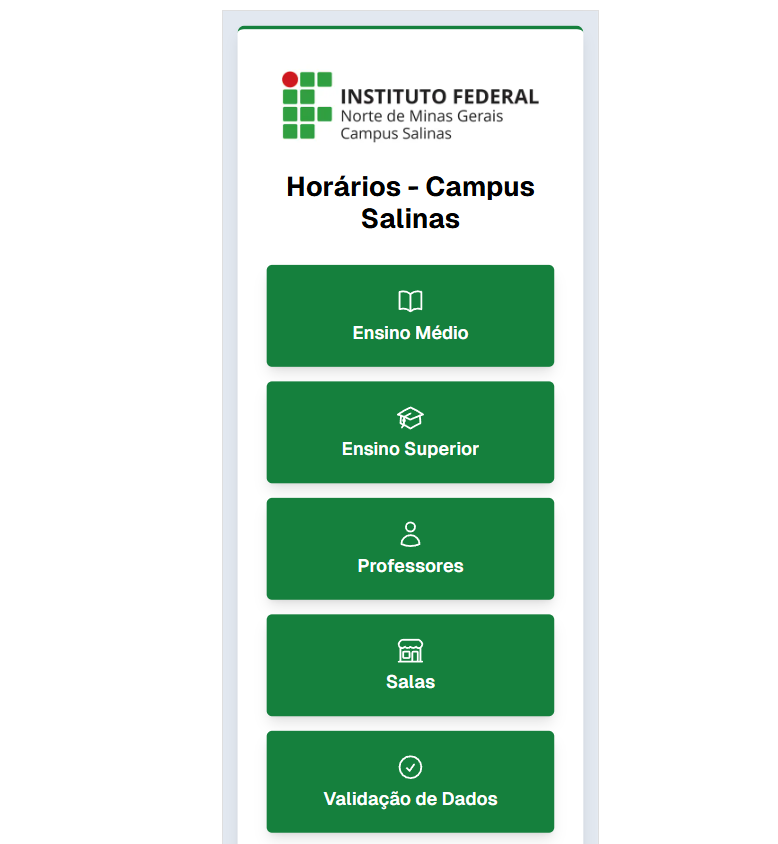
\includegraphics[width=0.9\textwidth]{figuras/front-16.png}
        \footnotesize Fonte: Elaborado pelo autor (2025)
    \end{minipage}
\end{frame}

\begin{frame}{Funcionalidades do Front-end}
    \begin{figure}
        \centering
        \vspace{-0.5cm}
        \caption{Busca de horários dos cursos técnicos e superiores}
        \vspace{-0.2cm}
        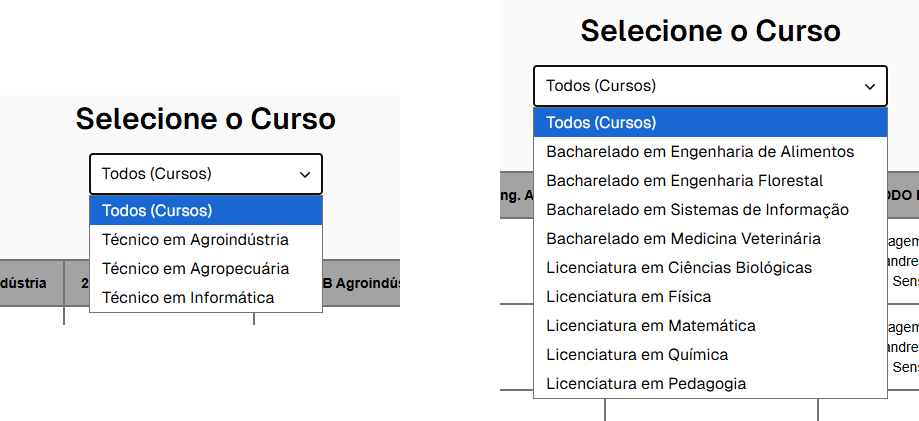
\includegraphics[width=1\textwidth]{figuras/front-17.png}
        \\ % Quebra de linha para separar a imagem da fonte
        \footnotesize Fonte: Elaborado pelo autor (2025)
    \end{figure}
\end{frame}

\begin{frame}{Funcionalidades do Front-end}
    \begin{minipage}{0.48\textwidth}
        \centering
        \captionof{figure}{Busca de horários de professores}
        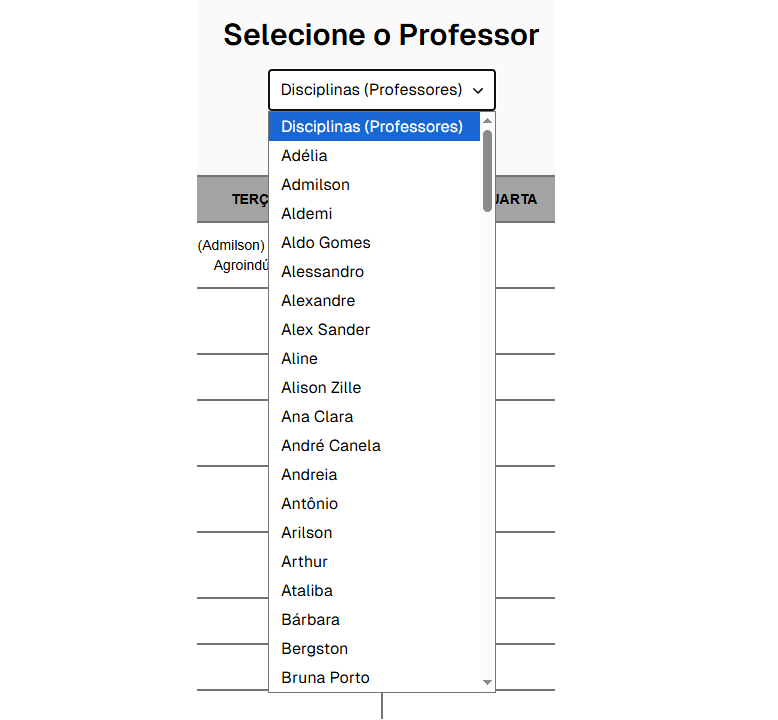
\includegraphics[width=1\textwidth]{figuras/front-18.png}
        \footnotesize Fonte: Elaborado pelo autor (2025)
    \end{minipage}
    \hfill
    \begin{minipage}{0.48\textwidth}
        \centering
        \captionof{figure}{Busca de horários de salas}
        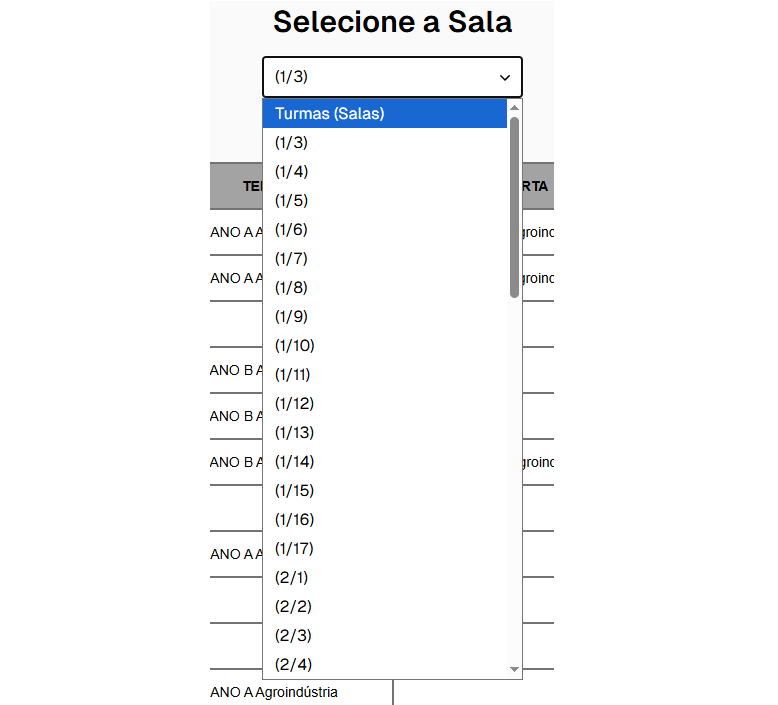
\includegraphics[width=1\textwidth]{figuras/front-19.png}
        \footnotesize Fonte: Elaborado pelo autor (2025)
    \end{minipage}
\end{frame}

\begin{frame}{Funcionalidades do Front-end}
    \begin{minipage}{0.48\textwidth}
        \centering
        \captionof{figure}{Download em PDF}
        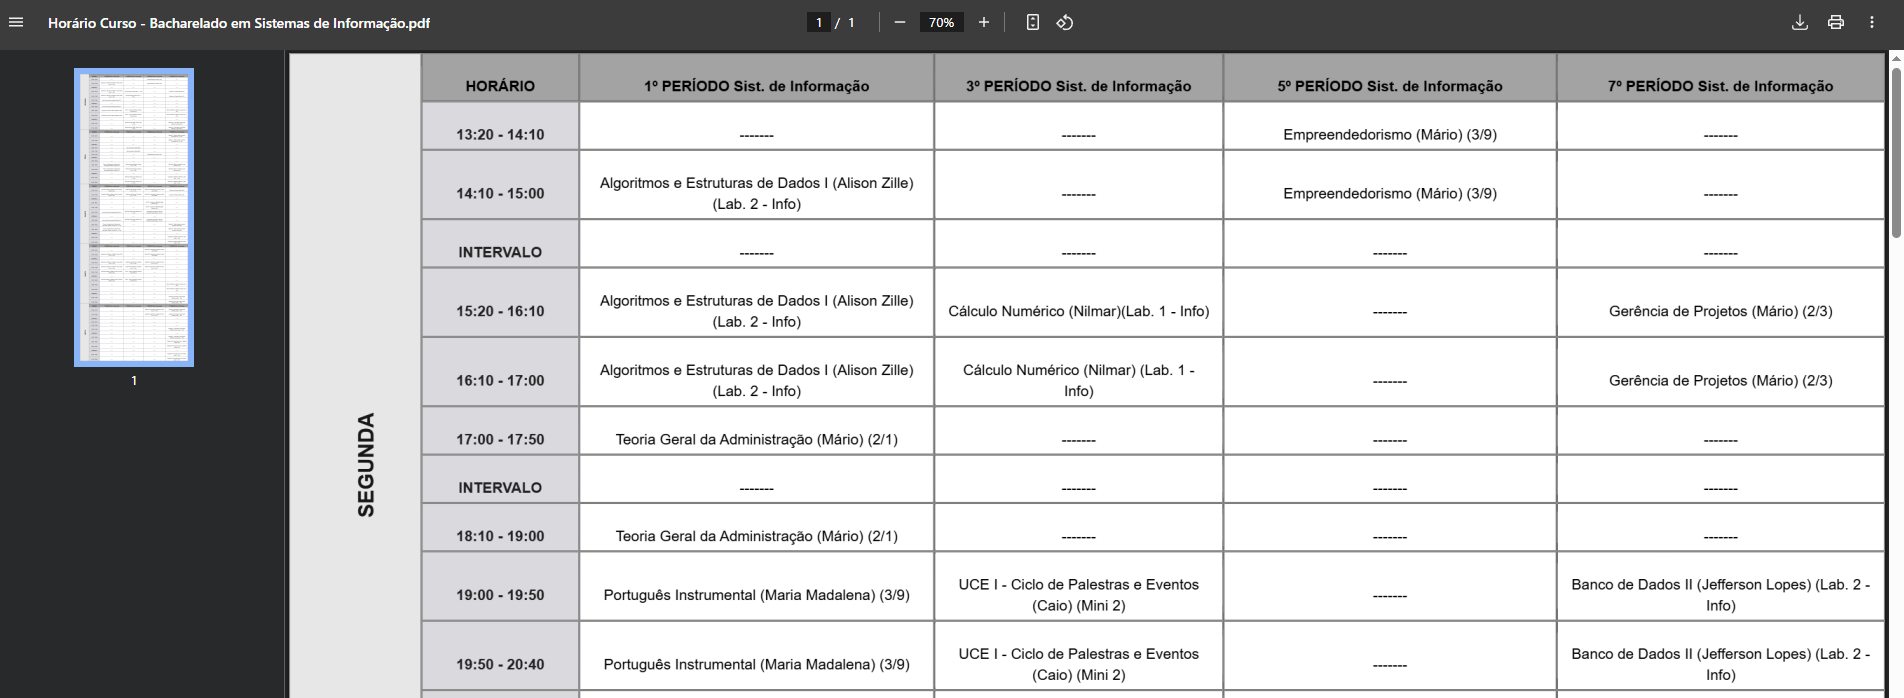
\includegraphics[width=1\textwidth]{figuras/front-20.png}
        \footnotesize Fonte: Elaborado pelo autor (2025)
    \end{minipage}
    \hfill
    \begin{minipage}{0.48\textwidth}
        \centering
        \captionof{figure}{Tela de login com credenciais incorretas}
        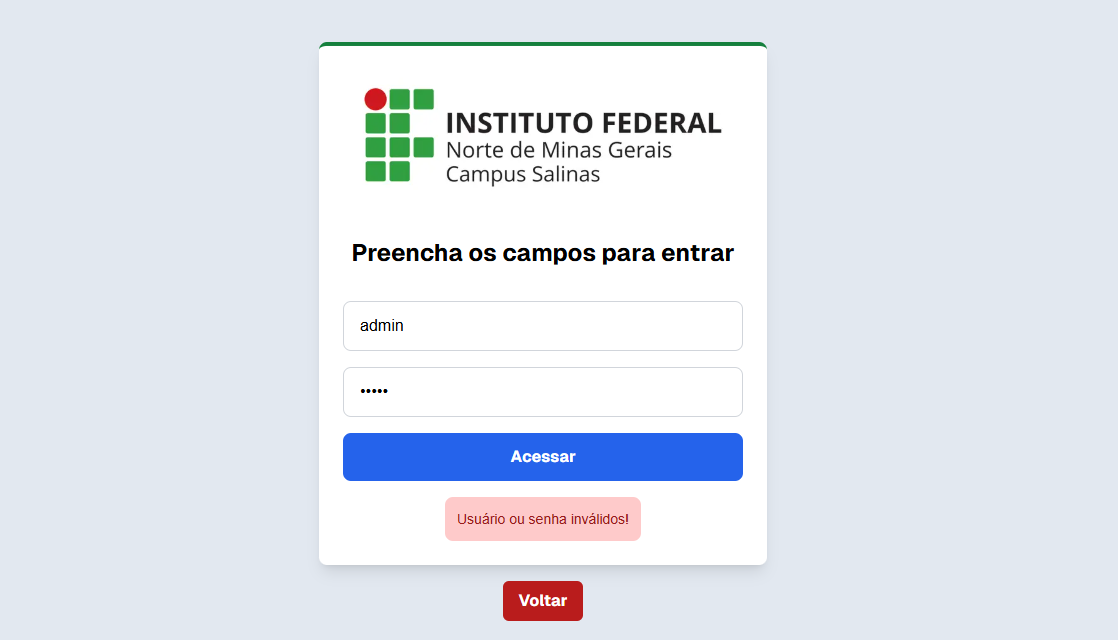
\includegraphics[width=1\textwidth]{figuras/front-21.png}
        \footnotesize Fonte: Elaborado pelo autor (2025)
    \end{minipage}
\end{frame}

\begin{frame}{Funcionalidades do Front-end}
    \begin{figure}
        \centering
        \vspace{-0.5cm}
        \caption{Tela de validação com resultado de sucesso}
        \vspace{-0.2cm}
        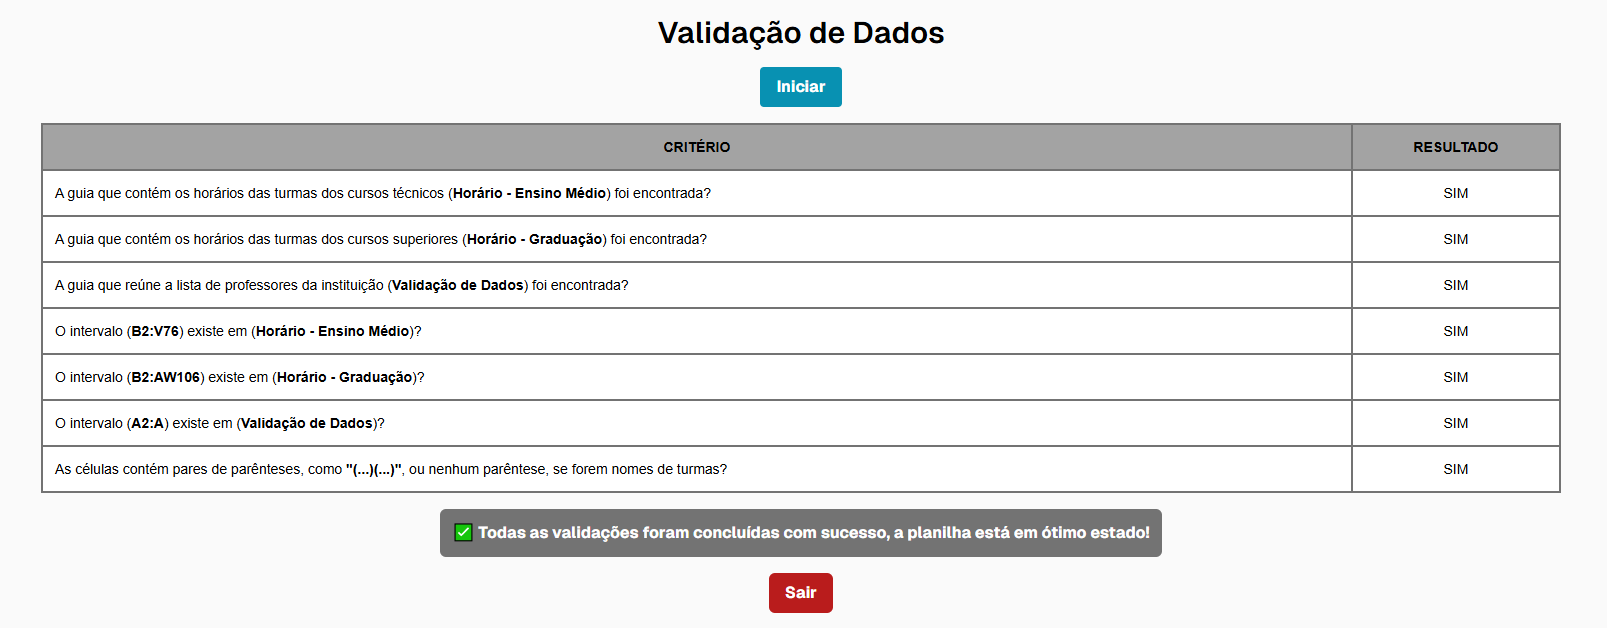
\includegraphics[width=1\textwidth]{figuras/front-22.png}
        \\ % Quebra de linha para separar a imagem da fonte
        \footnotesize Fonte: Elaborado pelo autor (2025)
    \end{figure}
\end{frame}

\begin{frame}{Funcionalidades do Front-end}
    \begin{figure}
        \centering
        \vspace{-0.5cm}
        \caption{Tela de validação com resultado mostrando inconsistências}
        \vspace{-0.2cm}
        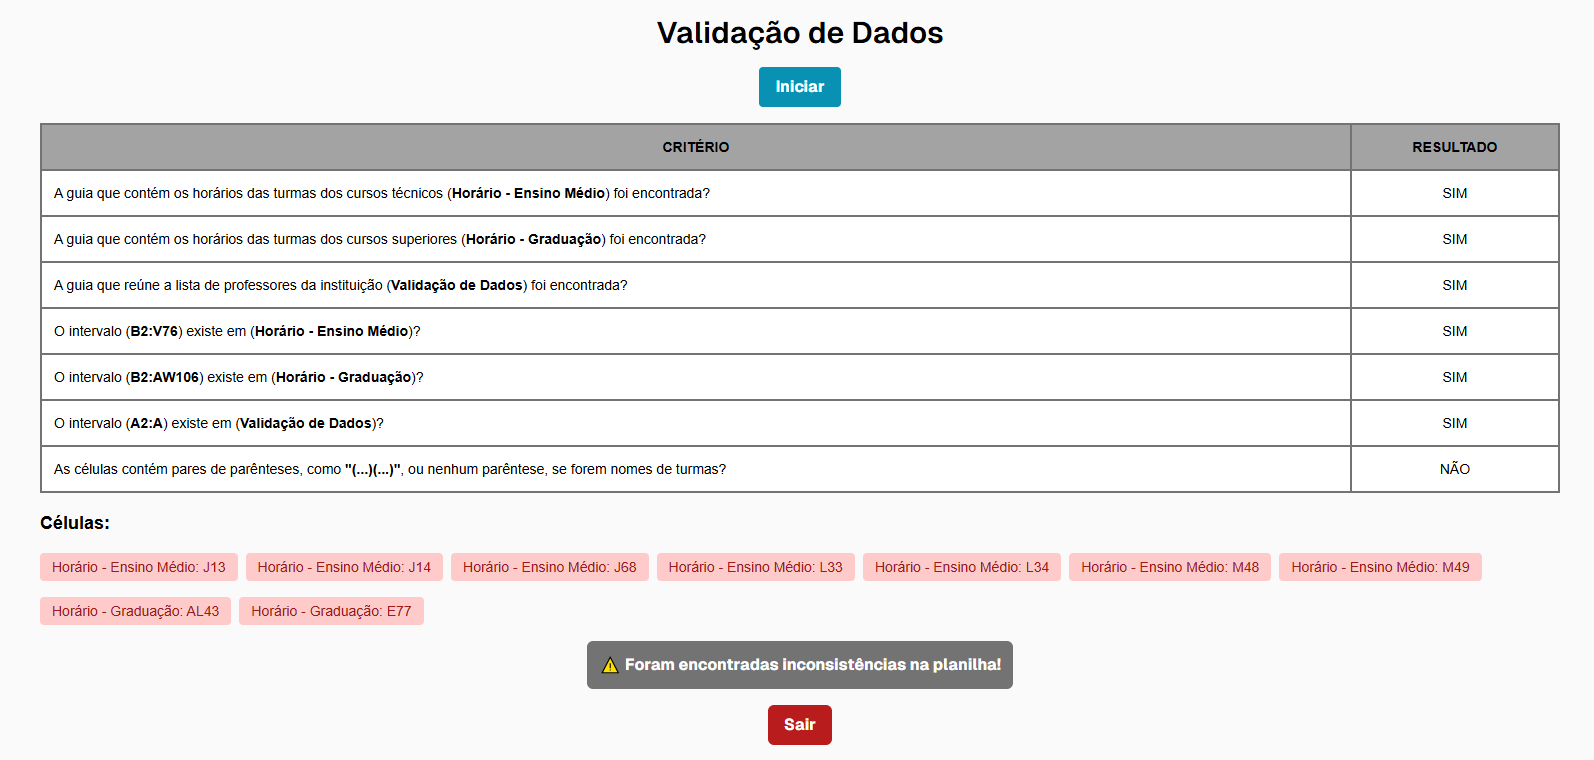
\includegraphics[width=1\textwidth]{figuras/front-23.png}
        \\ % Quebra de linha para separar a imagem da fonte
        \footnotesize Fonte: Elaborado pelo autor (2025)
    \end{figure}
\end{frame}

\begin{frame}{Funcionalidades do Front-end}
    \begin{figure}
        \centering
        \vspace{-0.5cm}
        \caption{Tela de validação com resultado de erro}
        \vspace{-0.2cm}
        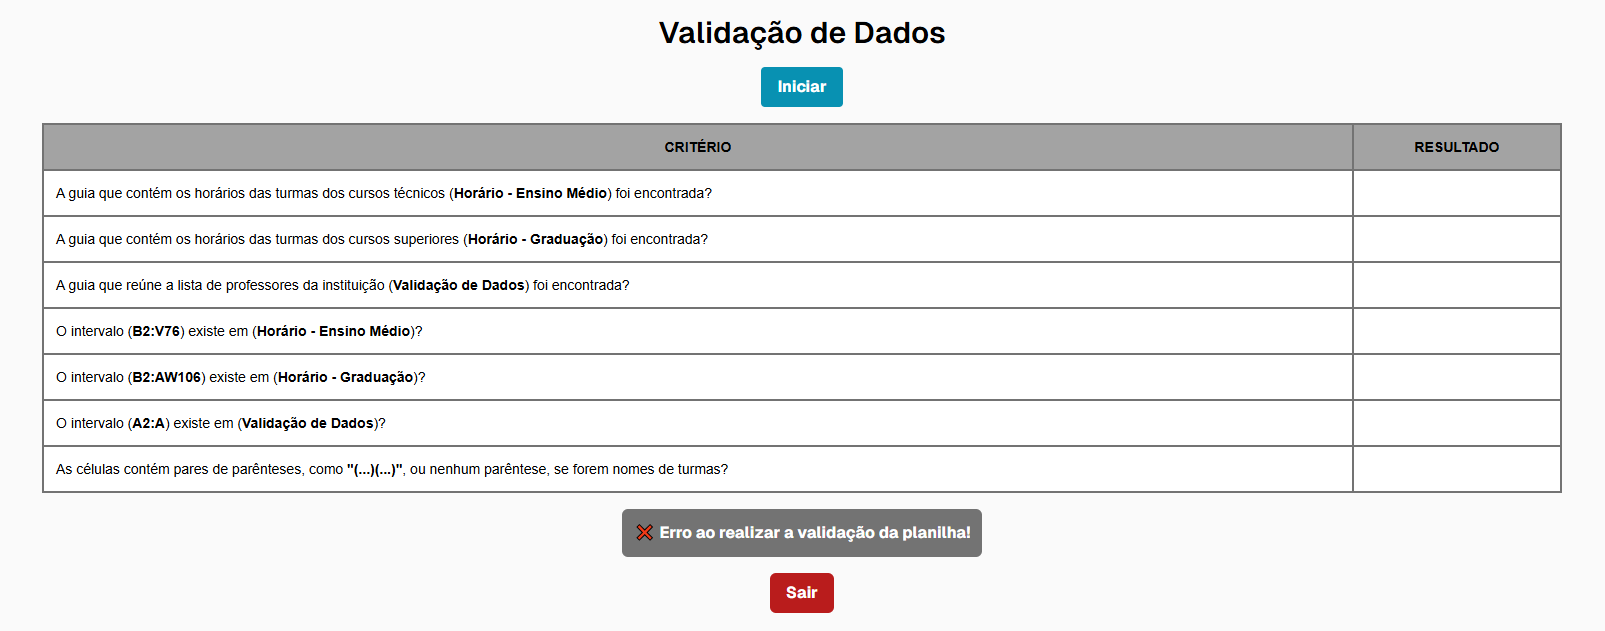
\includegraphics[width=1\textwidth]{figuras/front-24.png}
        \\ % Quebra de linha para separar a imagem da fonte
        \footnotesize Fonte: Elaborado pelo autor (2025)
    \end{figure}
\end{frame}

\begin{frame}{Back-end}
    \begin{itemize}
        \item Google Sheets como Banco de Dados: \vspace{0.5cm}
    \end{itemize}
    \begin{figure}
        \centering
        \vspace{-0.8cm}
        \caption{Guia ``Horário - Ensino Médio''}
        \vspace{-0.2cm}
        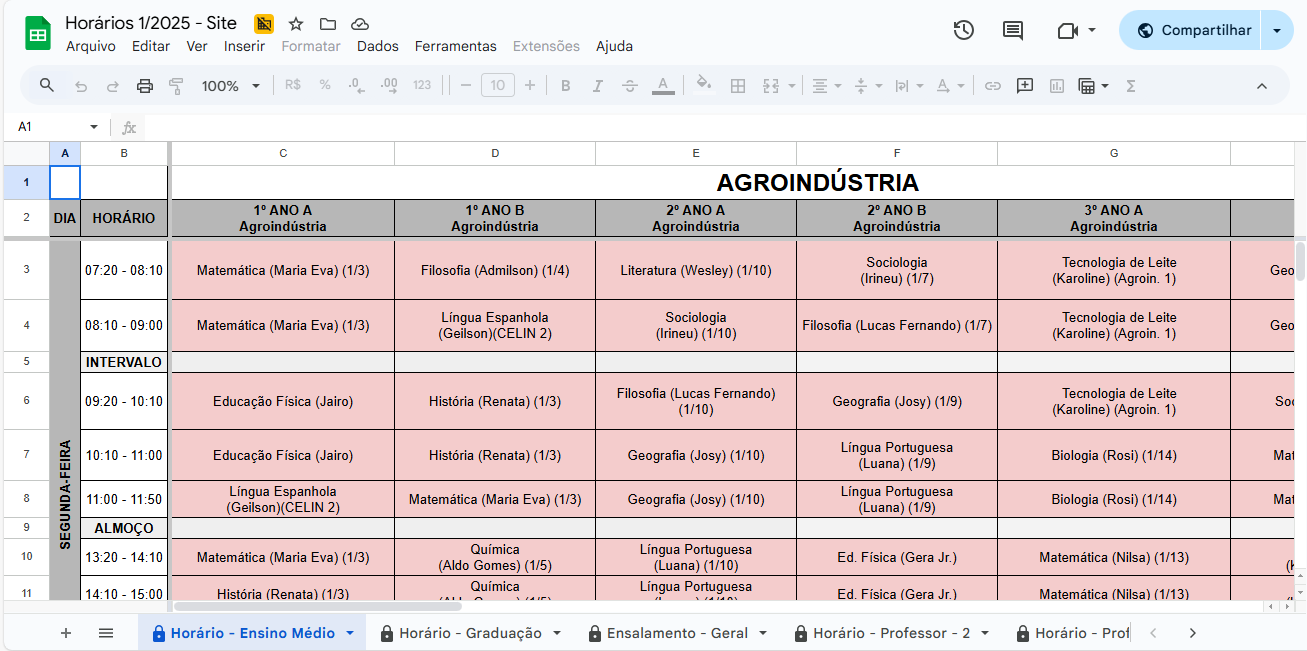
\includegraphics[width=1\textwidth]{figuras/plan-1.png}
        \\ % Quebra de linha para separar a imagem da fonte
        \footnotesize Fonte: Elaborado pelo autor (2025)
    \end{figure}
\end{frame}

\begin{frame}{Google Sheets como Banco de Dados}
    \begin{figure}
        \centering
        \vspace{-0.5cm}
        \caption{Guia ``Horário - Graduação''}
        \vspace{-0.2cm}
        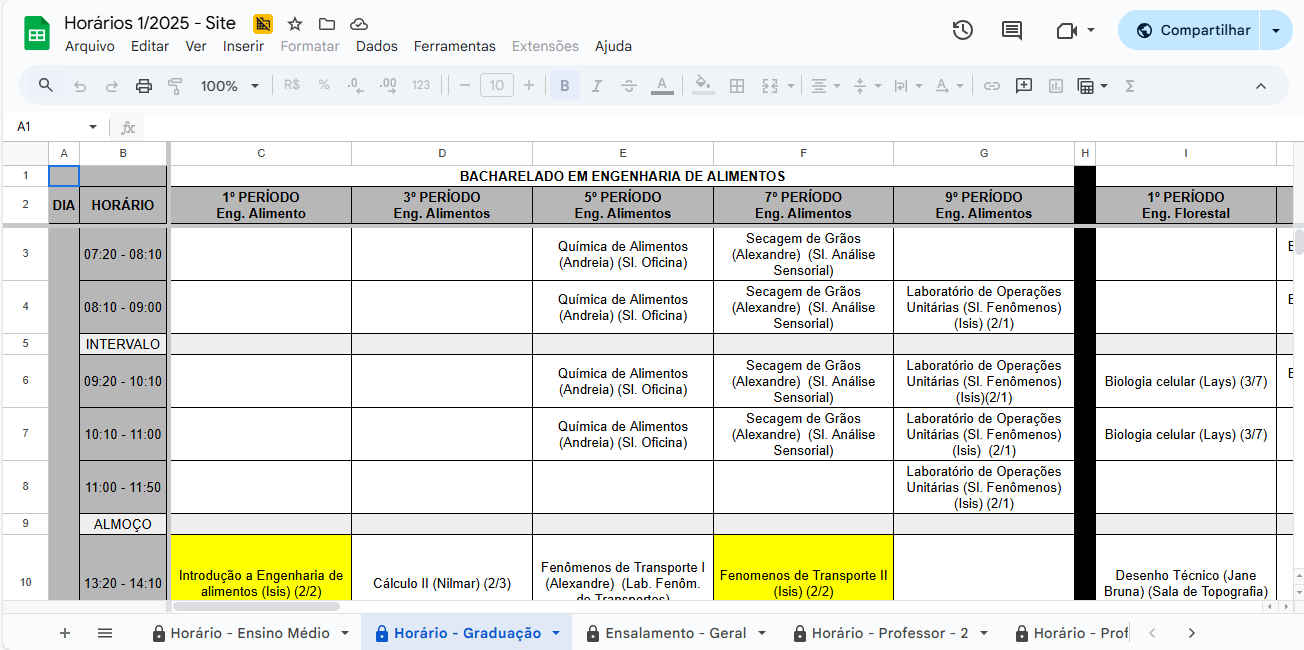
\includegraphics[width=1\textwidth]{figuras/plan-2.png}
        \\ % Quebra de linha para separar a imagem da fonte
        \footnotesize Fonte: Elaborado pelo autor (2025)
    \end{figure}
\end{frame}

\begin{frame}{Google Sheets como Banco de Dados}
    \begin{figure}
        \centering
        \vspace{-0.5cm}
        \caption{Guia ``Validação de Dados''}
        \vspace{-0.2cm}
        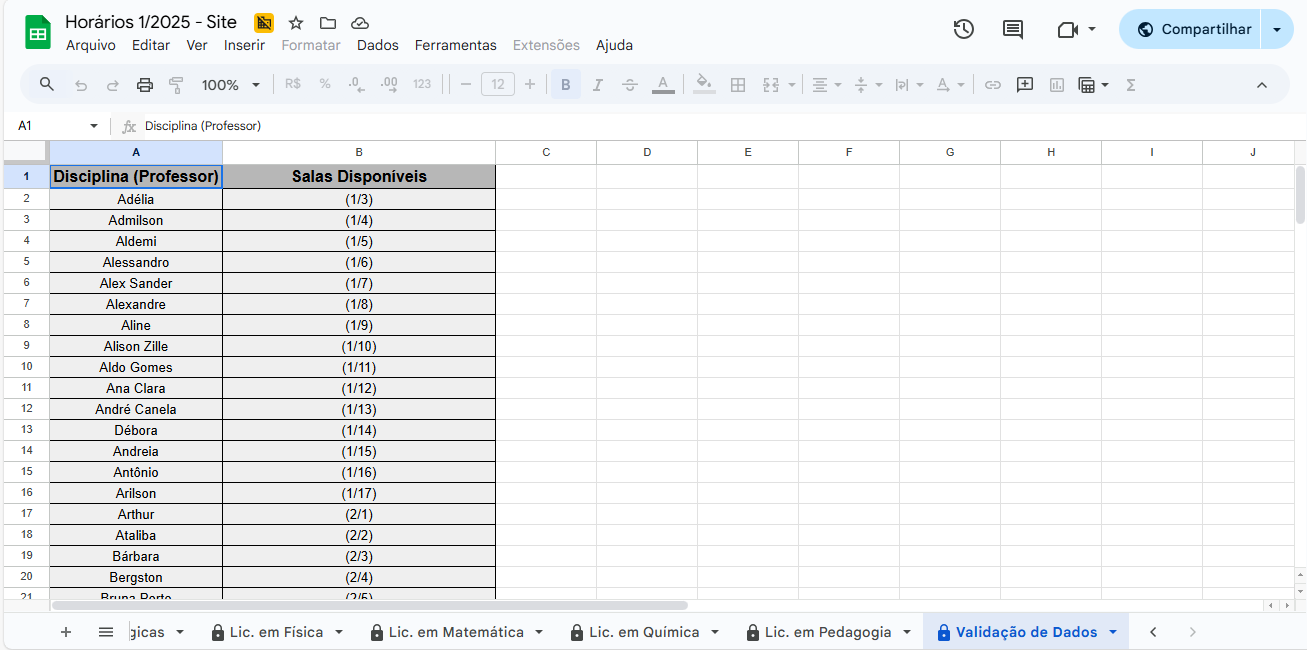
\includegraphics[width=1\textwidth]{figuras/plan-3.png}
        \\ % Quebra de linha para separar a imagem da fonte
        \footnotesize Fonte: Elaborado pelo autor (2025)
    \end{figure}
\end{frame}

\begin{frame}{Google Sheets como Banco de Dados}
    \begin{figure}
        \centering
        \vspace{-0.5cm}
        \caption{Guia ``Login''}
        \vspace{-0.2cm}
        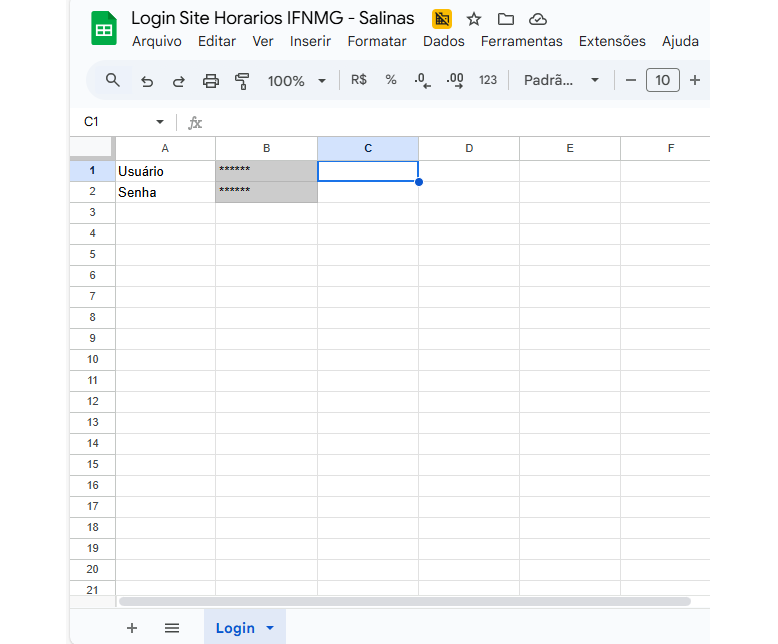
\includegraphics[width=0.85\textwidth]{figuras/plan-4.png}
        \\ % Quebra de linha para separar a imagem da fonte
        \footnotesize Fonte: Elaborado pelo autor (2025)
    \end{figure}
\end{frame}

\begin{frame}{Estrutura do Back-end}
    \begin{figure}
        \centering
        \vspace{-0.5cm}
        \caption{Estrutura do back-end}
        \vspace{-0.2cm}
        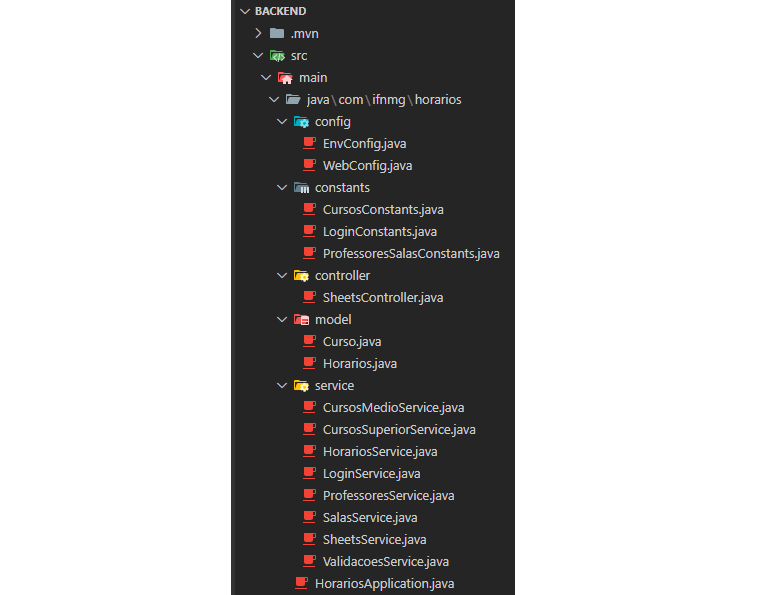
\includegraphics[width=1\textwidth]{figuras/back-1.png}
        \\ % Quebra de linha para separar a imagem da fonte
        \footnotesize Fonte: Elaborado pelo autor (2025)
    \end{figure}
\end{frame}

\begin{frame}{Funcionalidades do Back-end}
    \begin{itemize}
        \item Estabelecer a conexão com a API do Google Sheets
    \end{itemize}
    \begin{figure}
        \centering
        \vspace{-0.4cm}
        \caption{Classe ``SheetsService.java''}
        \vspace{-0.2cm}
        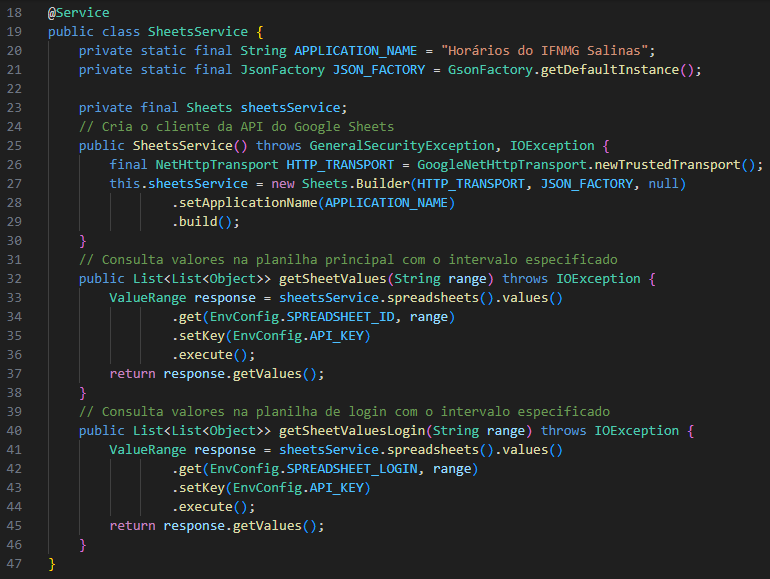
\includegraphics[width=0.95\textwidth]{figuras/back-2.png}
        \\ % Quebra de linha para separar a imagem da fonte
        \footnotesize Fonte: Elaborado pelo autor (2025)
    \end{figure}
\end{frame}

\begin{frame}{Funcionalidades do Back-end}
    \begin{itemize}
        \item Disponibilizar endpoints REST
    \end{itemize}
    \begin{figure}
        \centering
        \vspace{-0.3cm}
        \caption{Endpoint de consulta dos horários dos cursos técnicos}
        \vspace{-0.2cm}
        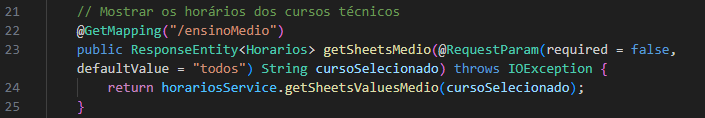
\includegraphics[width=1\textwidth]{figuras/back-3.png}
        \\ % Quebra de linha para separar a imagem da fonte
        \footnotesize Fonte: Elaborado pelo autor (2025)
    \end{figure}
    \begin{figure}
        \centering
        \vspace{-0.5cm}
        \caption{Endpoint de consulta dos horários dos cursos superiores}
        \vspace{-0.2cm}
        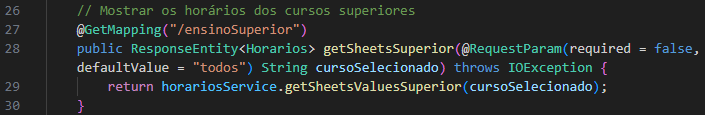
\includegraphics[width=1\textwidth]{figuras/back-4.png}
        \\ % Quebra de linha para separar a imagem da fonte
        \footnotesize Fonte: Elaborado pelo autor (2025)
    \end{figure}
\end{frame}

\begin{frame}{Funcionalidades do Back-end}
    \begin{figure}
        \centering
        \vspace{-0.3cm}
        \caption{Endpoint de consulta dos horários dos professores}
        \vspace{-0.2cm}
        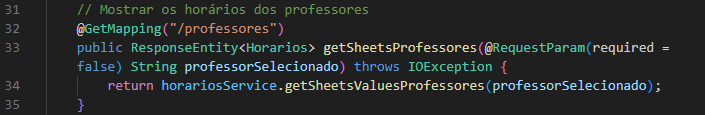
\includegraphics[width=1\textwidth]{figuras/back-5.png}
        \\ % Quebra de linha para separar a imagem da fonte
        \footnotesize Fonte: Elaborado pelo autor (2025)
    \end{figure}
    \begin{figure}
        \centering
        \vspace{-0.5cm}
        \caption{Endpoint de consulta dos horários de ocupação das salas}
        \vspace{-0.2cm}
        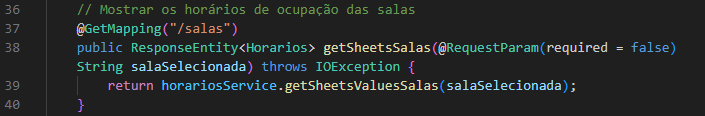
\includegraphics[width=1\textwidth]{figuras/back-6.png}
        \\ % Quebra de linha para separar a imagem da fonte
        \footnotesize Fonte: Elaborado pelo autor (2025)
    \end{figure}
\end{frame}

\begin{frame}{Funcionalidades do Back-end}
    \begin{figure}
        \centering
        \vspace{-0.3cm}
        \caption{Endpoint de consulta das permissões para visualizar validação da planiha}
        \vspace{-0.2cm}
        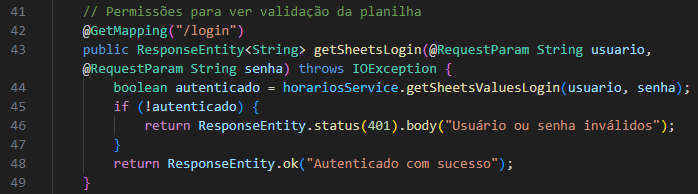
\includegraphics[width=0.9\textwidth]{figuras/back-7.png}
        \\ % Quebra de linha para separar a imagem da fonte
        \footnotesize Fonte: Elaborado pelo autor (2025)
    \end{figure}
    \begin{figure}
        \centering
        \vspace{-0.5cm}
        \caption{Endpoint de consulta para validar dados da planilha}
        \vspace{-0.2cm}
        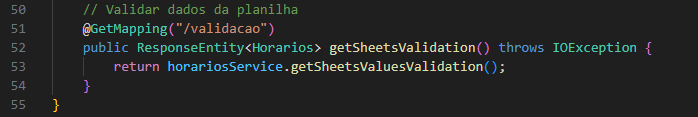
\includegraphics[width=1\textwidth]{figuras/back-8.png}
        \\ % Quebra de linha para separar a imagem da fonte
        \footnotesize Fonte: Elaborado pelo autor (2025)
    \end{figure}
\end{frame}

\begin{frame}{Deploy}
    \begin{itemize}
        \item Front-end:
    \end{itemize}
    \begin{figure}
        \centering
        \vspace{-0.3cm}
        \caption{Deploy do front-end da plataforma na Vercel}
        \vspace{-0.2cm}
        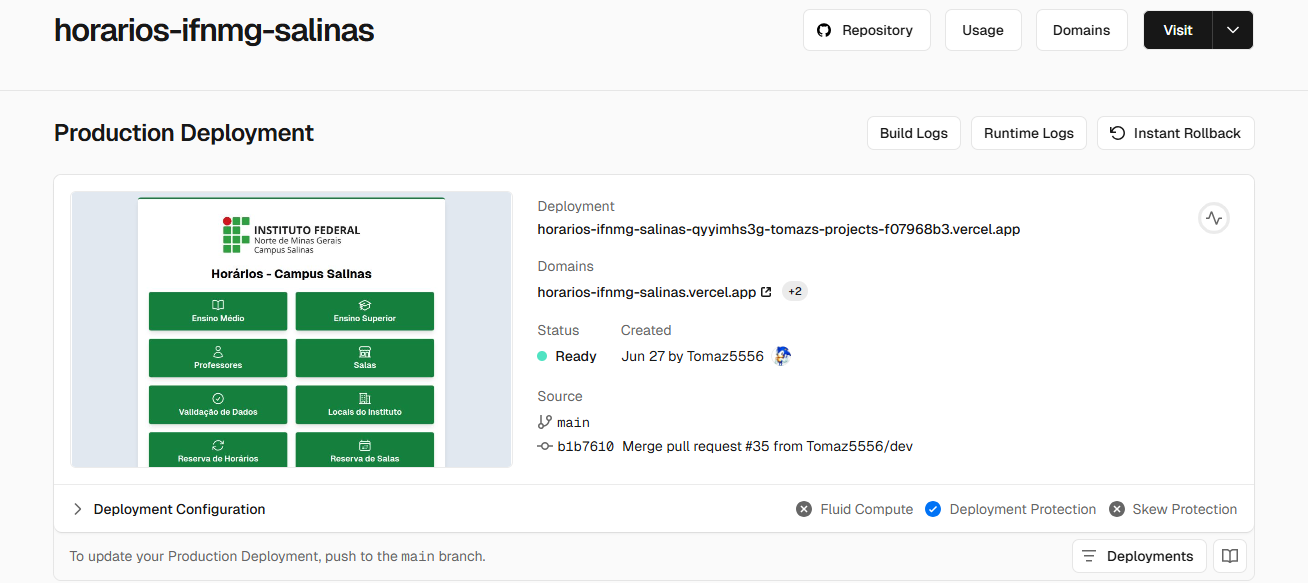
\includegraphics[width=1\textwidth]{figuras/deploy-1.png}
        \\ % Quebra de linha para separar a imagem da fonte
        \footnotesize Fonte: Elaborado pelo autor (2025)
    \end{figure}
\end{frame}

\begin{frame}{Deploy}
    \begin{itemize}
        \item Back-end:
    \end{itemize}
    \begin{figure}
        \centering
        \vspace{-0.3cm}
        \caption{Deploy do back-end da plataforma na Koyeb}
        \vspace{-0.2cm}
        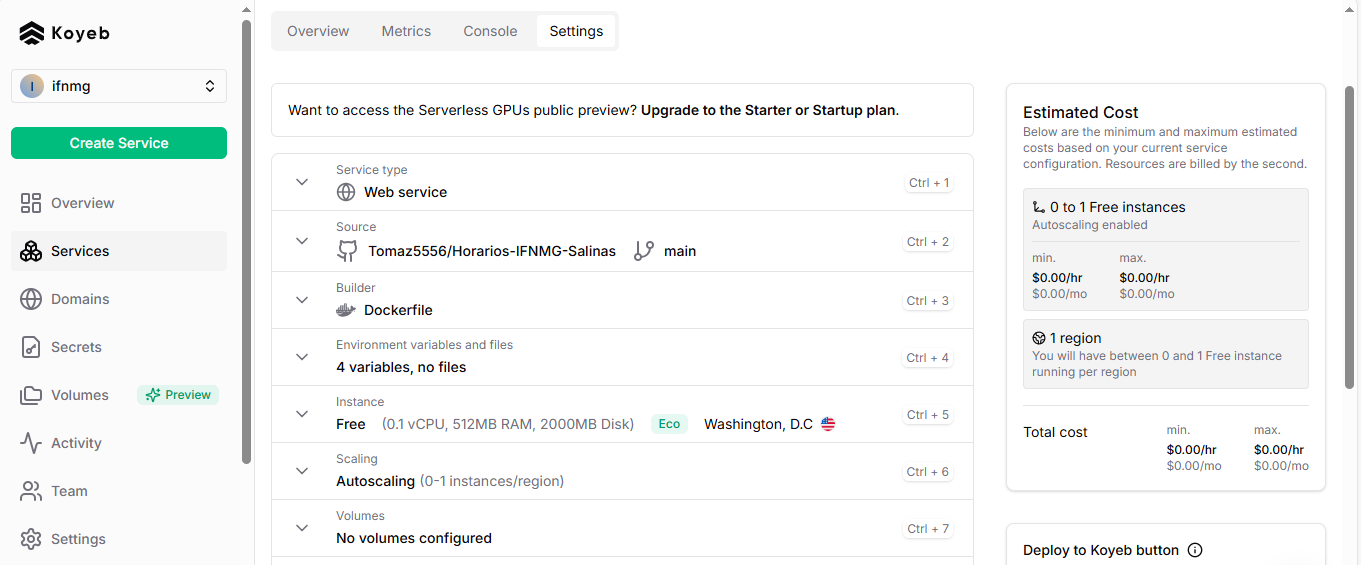
\includegraphics[width=1\textwidth]{figuras/deploy-2.png}
        \\ % Quebra de linha para separar a imagem da fonte
        \footnotesize Fonte: Elaborado pelo autor (2025)
    \end{figure}
\end{frame}

\begin{frame}{Documentação}
    \begin{itemize}
        \item Documentação técnica elaborada para a planilha utilizada como banco de dados do sistema.
    \end{itemize}
    \begin{minipage}{0.48\textwidth}
        \centering
        \captionof{figure}{Instruções para desenvolvedores}
        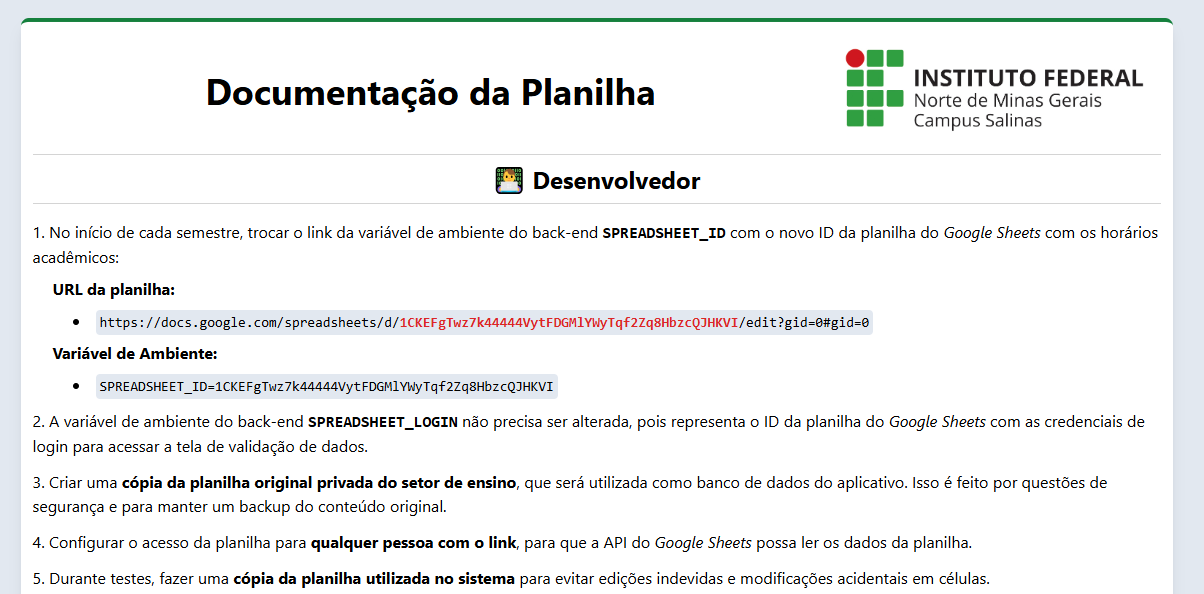
\includegraphics[width=1\textwidth]{figuras/doc-1.png}
        \footnotesize Fonte: Elaborado pelo autor (2025)
    \end{minipage}
    \hfill
    \begin{minipage}{0.48\textwidth}
        \centering
        \captionof{figure}{Instruções para administradores da planilha}
        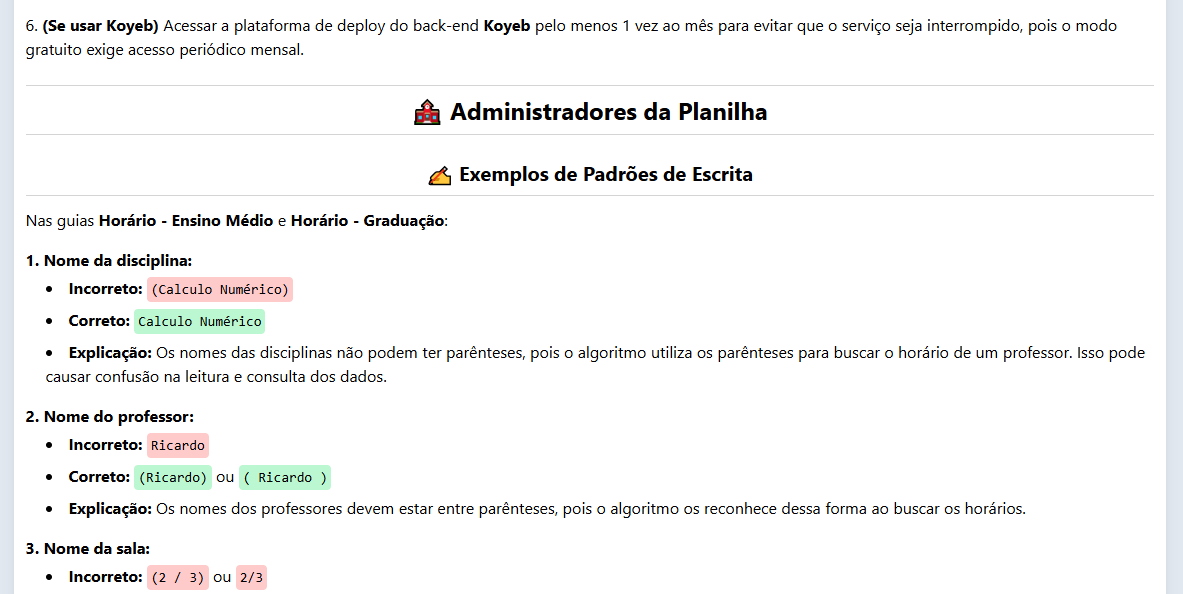
\includegraphics[width=1\textwidth]{figuras/doc-2.png}
        \footnotesize Fonte: Elaborado pelo autor (2025)
    \end{minipage}
\end{frame}

\begin{frame}{Documentação}
    \begin{minipage}{0.48\textwidth}
        \centering
        \captionof{figure}{Explicação das guias e intervalos de células}
        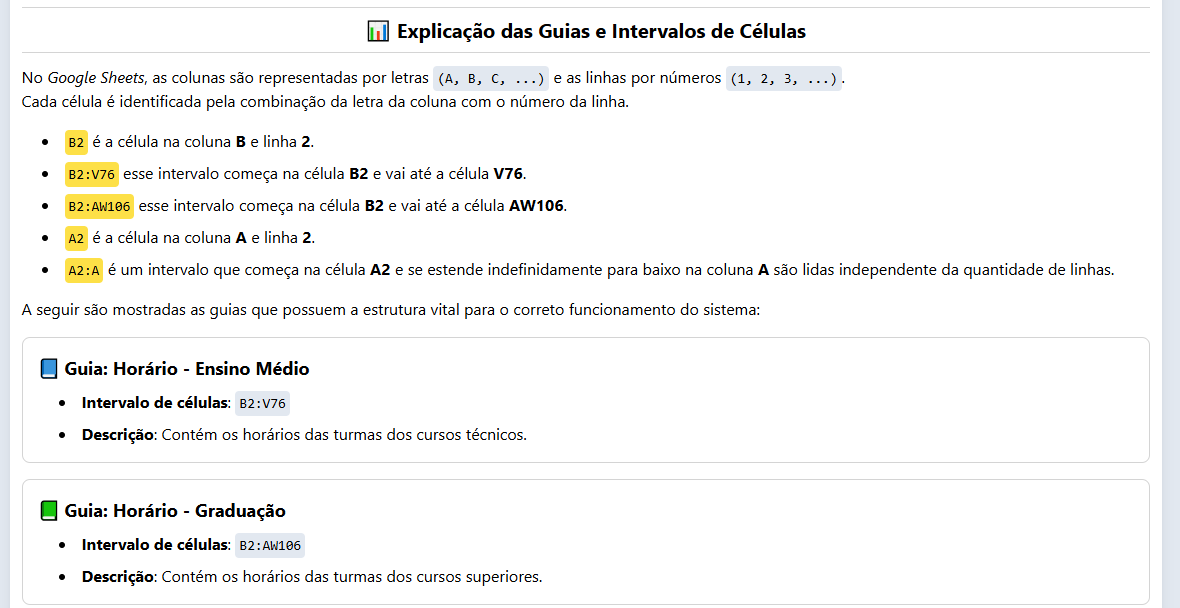
\includegraphics[width=1\textwidth]{figuras/doc-3.png}
        \footnotesize Fonte: Elaborado pelo autor (2025)
    \end{minipage}
    \hfill
    \begin{minipage}{0.48\textwidth}
        \centering
        \captionof{figure}{Observação sobre mudanças estruturais}
        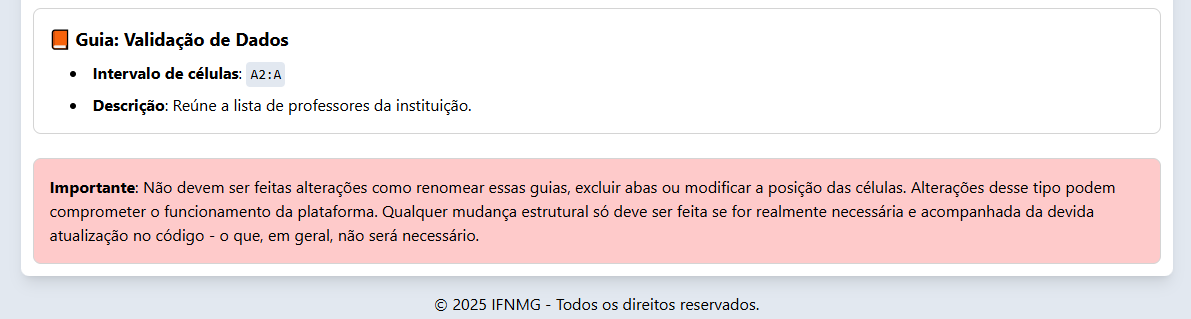
\includegraphics[width=1\textwidth]{figuras/doc-4.png}
        \footnotesize Fonte: Elaborado pelo autor (2025)
    \end{minipage}
\end{frame}